\section{Z80 Minimalsystem}
\label{sec:z80}
\subsection{Projektidee}
\label{sec:z80-idee}
\subsubsection{Warum ein Z80 Minimalsystem?}
\label{sec:z80-warum}
Das Z80 Minimalsystem wurde für die Anwendung im Laborunterricht entworfen, wo es gemeinsam mit einem Logikanalysator eingesetzt wird, um Bustimings des Z80 zu erfassen und zu analysieren. Die Wahl fiel auf den Z80, da der Befehlssatz und der Aufbau der „von-Neumann-Architektur“ bereits durch den Theorieunterricht bekannt ist und die Möglichkeit der Aufzeichnung der Timings der systeminternen Busse besteht, da es sich um ein Mikroprozessorsystem und nicht um einen Mikrocontroller handelt.

Das Lehrsystem Microprofessor $\micro$PF 1, welches im DIC-Unterricht (Digitale Systeme) verwendet wird, arbeitet ebenfalls mit einer Z80 CPU und stellt die Grundlage für das Z80 Minimalsystem dar. Der Lerncomputer $\micro$PF 1 ist auf eine möglichst einfache Programmierbarkeit ausgelegt und eignet sich deshalb bestens für das Testen neu entwickelter Programme. Hingegen sind im Laborunterricht kurze Vorbereitungszeiten gefragt, weshalb das Minimalsystem keine direkte Programmiermöglichkeit wie der $\micro$PF 1 besitzt. Der $\micro$PF 1 verfügt über eine Tastatur und ein Display, um mithilfe eines Monitorprogramms Programme in den SRAM zu schreiben, sie auszuführen und sie zu debuggen. Beim Z80 Minimalsystem wird das Programm auf einem PC erstellt und übersetzt und mithilfe eines Programmiergeräts fix in einem EPROM abgelegt. Weiters verfügt das Minimalsystem im Gegensatz zum $\micro$PF 1 über einen DMA Controller für direkte Zugriffe der Peripherie auf den Speicher und über eine RS232-Schnittstelle. Um ein Bustiming aufzeichnen zu können, sind Datenbus, Adressbus und Steuerbus extra an Stiftleisten herausgeführt.

\subsection{Aufbau}
\label{sec:z80-aufbau}
\subsubsection{Blockschaltbild des Gesamtsystems}
\label{sec:z80-bsb}
\fig{z80-bsb}{Z80 Blockschaltbild}{Blockschaltbild}{\textwidth}{Reischl/img/z80-bsb}

Wie im obigen Blockschaltbilde zu sehen ist, besteht das System aus einer CPU, dem Speicherwerk und der Peripherie. Die einzelnen Baugruppen des Mikroprozessorsystems sind miteinander mit dem 16 Bit breiten unidirektionalen Adressbus, den 8 Bit breiten bidirektionalen Datenbus und dem Steuerbus verbunden.

\fig{z80-foto}{Z80 Fotografie}{Fotografie des Minimalsystems}{\textwidth}{Reischl/img/z80-foto}
\fig{z80-draufsicht}{Z80 Draufsicht}{Draufsicht des Minimalsystems}{\textwidth}{Reischl/img/z80-draufsicht}

In diesen beiden Abbildungen ist zu sehen, wo welche Komponenten des Z80 Minimalsystems platziert sind, wie diese aussehen und wie sie benannt werden. Die Bezeichnungen der einzelnen Teile können dem zweiten Bild entnommen werden, eine Beschreibung ist im nächsten Kapitel zu finden.

% \subsubsection{Speicherzugriff durch die Peripherie}
% \begin{figure}[htb]
%     \centering
%     \subfloat{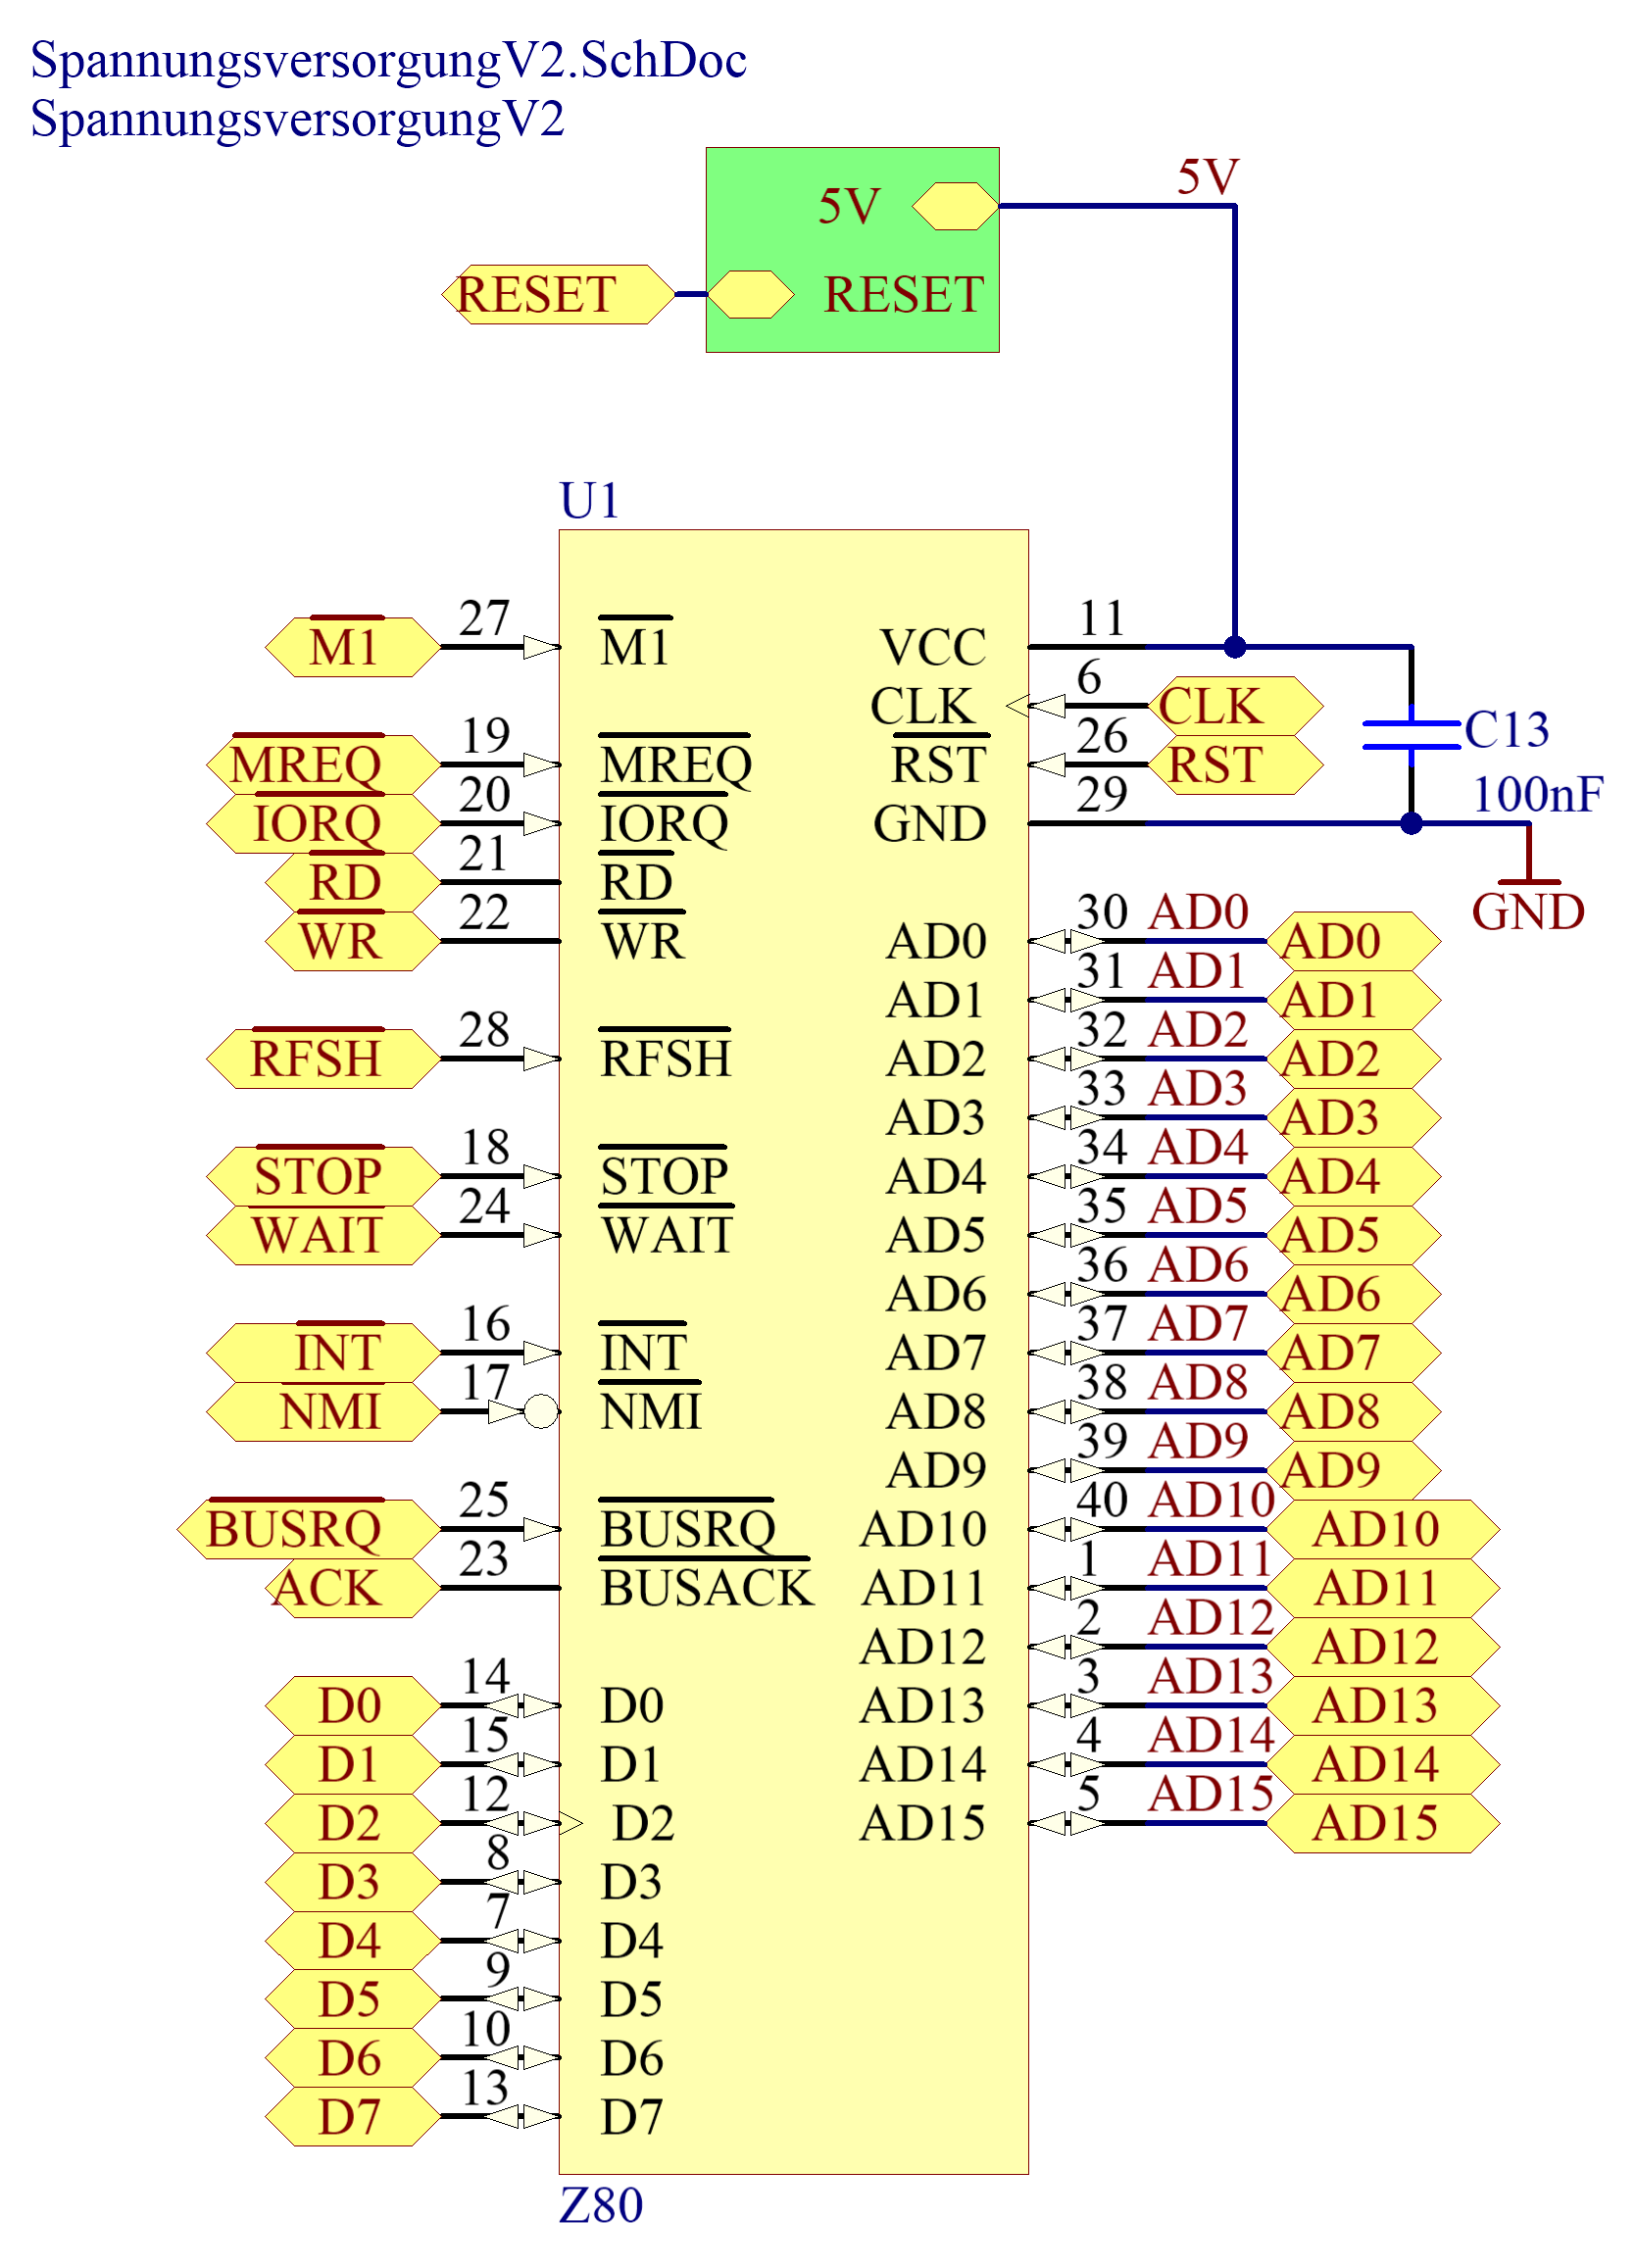
\includegraphics[width=.4\linewidth]{Reischl/img/z80-speicherper-1}}\qquad
%     \subfloat{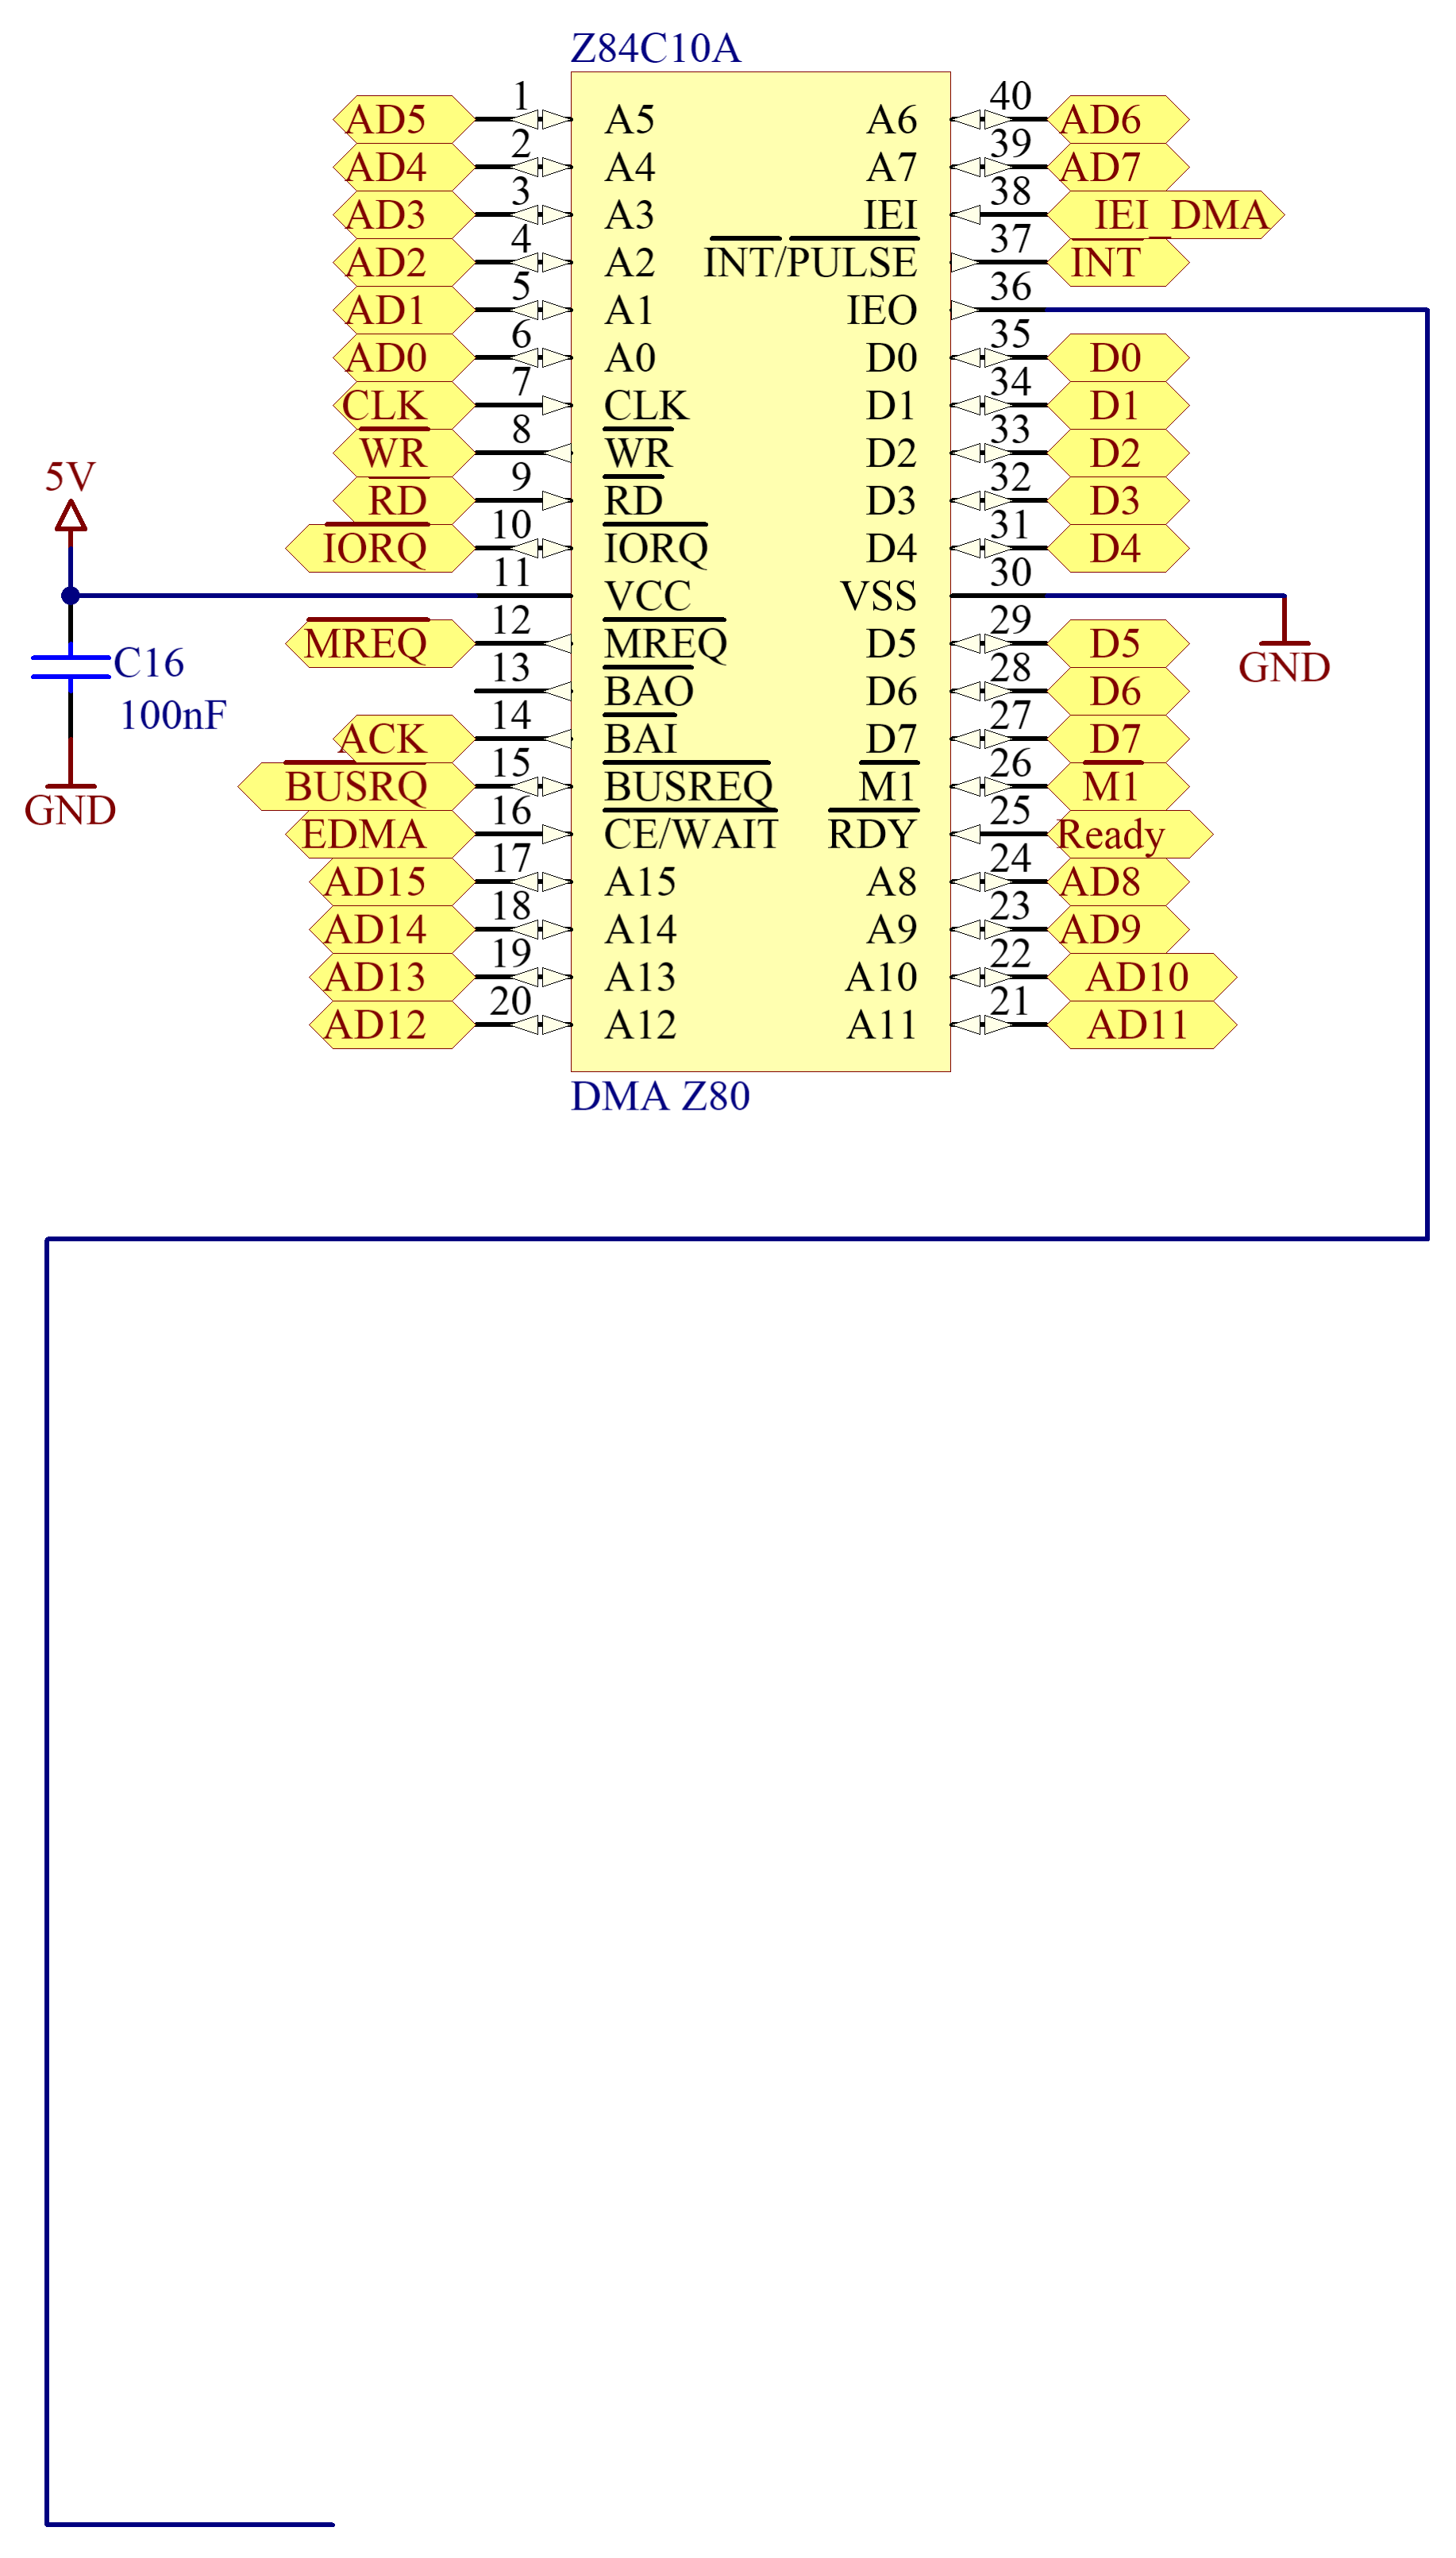
\includegraphics[width=.4\linewidth]{Reischl/img/z80-speicherper-2}}\qquad
%     \caption[Z80 Speicherdirektzugriff]{Speicherdirektzugriff}
%     \label{fig:z80-zeit}
% \end{figure}
% Der DMA Controller ermöglicht Speicherdirektzugriffe und Abarbeitung von Daten mit einer $2^n$ fachen Frequenz des Systemtaktes. Der DMAC besitzt wie der SIO und der CTC die Möglichkeit, einen Interrupt (INT) auszulösen und ist somit Teil der Daisy Chain (IEI). Bei einer Datenübertragung, die nicht von der CPU selbst vorgenommen wird, ist es wichtig, darauf zu achten, dass der Daten- und Adressbus nicht gleichzeitig von mehreren Baugruppen verwendet wird. Dies wird durch das Acknowledge (BAI bzw. ACK) überprüft, über den Busrequest (BUSREQ) wird der Übertragungsvorgang gesteuert. I/O Request, Memory Request, Read und Write dienen der Steuerung des Speicher- bzw. Peripheriezugriffs, die Funktion von IEI ist der Beschreibung des SIO zu entnehmen. Detailliertere Informationen sind im Z80 Family CPU Peripherals User Manual \cite{z80:periph} zu finden.

\subsection{Baugruppen}
\label{sec:z80-baugruppen}
\subsubsection{Spannungsversorgung}
Die gesamte Hardware, die beim Z80 Minimalsystem zum Einsatz kommt, benötigt eine Betriebsspannung von 5V Gleichspannung. Die erlaubte Schwankungsbreite der Spannung liegt bei allen systemspezifischen Komponenten und bei den verwendeten Logikgattern laut den einzelnen Datenblättern in einem Bereich von 4,75V bis 5,25V. Die Anforderung an die Spannungsversorgung war neben der guten Verfügbarkeit der einzelnen Versorgungsarten ein möglichst geringer Störungsanteil bei gleichzeitig einfacher Umsetzbarkeit. Deshalb fiel die Wahl auf 2 verschiedene Versorgungsmöglichkeiten: Die erste Möglichkeit ist die Versorgung mittels Netzteil mit Linearregler auf dem Minimalsystem. Bei der zweiten Variante handelt es sich um eine USB-Versorgung, deren Schnittstelle im Gegensatz zu den vorherigen Versionen nicht als Micro-USB ausgeführt ist, sondern als USB Typ B. Dadurch wird eine bessere mechanische Stabilität der Steckverbindung ermöglicht, außerdem werden USB-B Kabel mit größeren Leitungsquerschnitten angeboten, wodurch der Spannungsabfall an der Versorgung so weit reduziert werden kann, dass die Untergrenze von 4,75V Betriebsspannung selbst bei der Verwendung von TTL-Logik anstatt der aktuell verwendeten NMOS bzw. CMOS-Technologie eingehalten werden kann.

\fig{z80-spannung}{Z80 Spannungsversorgung}{Spannungsversorgung}{\textwidth}{Reischl/img/z80-spannung}

\subsubsubsection{Fixspannungsregler/Netzversorgung}
Bei dem verwendeten Fixspannungsregler vom Typ L7805CV handelt es sich um einen Linearregler des Herstellers ST Microelectronics. Dieser verfügt über eine Ausgangsspannung von 5V bei einem Maximalstrom von 1A. Die minimale Spannung am Ausgang liegt bei 4,8V, das Maximum beträgt 5,2V. Am Eingang dürfen abhängig vom Ausgangsstrom, der daraus resultierenden Verlustleistung und der Tatsache, ob und welcher Kühlkörper verwendet wird, theoretisch bis zu 35V anliegen. Um einen störungsfreien Betrieb zu gewährleisten, ist der Linearregler entsprechend Datenblatt am Eingang mit einer Kapazität von 330nF und am Ausgang mit 100nF zu versehen.
\begin{figure}[H]
    \subfloat[Gehäuse]{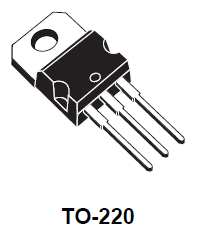
\includegraphics[width=.4\linewidth]{Reischl/img/z80-lin-1}}\qquad
    \subfloat[Pinning]{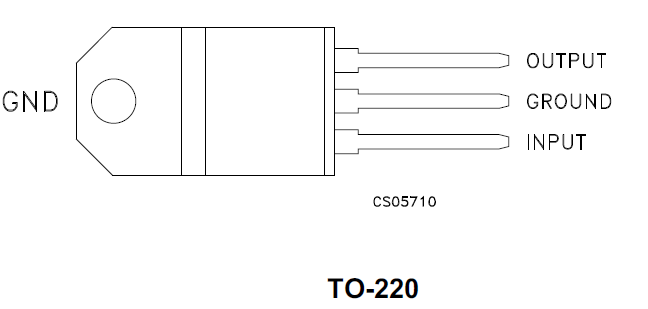
\includegraphics[width=.4\linewidth]{Reischl/img/z80-lin-2}}\qquad
    \caption[Z80 Linearregler Gehäuse und Pinning]{Linearregler Gehäuse und Pinning \cite{z80:lin}}
    \label{fig:z80-lin-1}
\end{figure}
Der am Minimalsystem verbaute Fixspannungsregler wurde am Eingang um einen Brückengleichrichter ergänzt, um einer Verpolung entgegenzuwirken und das System vor etwaigen Schäden durch den Betrieb mit einem AC-Netzteil zu schützen. Wenn möglich, sollte aber ein DC-Netzteil mit einer Ausgangsspannung 9V verwendet werden, um die Dropout Voltage nicht zu unterschreiten und gleichzeitig die Verlustleistung gering zu halten, da kein Kühlkörper verbaut wurde. Schnittstelle zwischen Minimalsystem und Netzteil bildet ein Niedervoltsteckverbinder, auch als PowerJack bezeichnet. Der verwendete Hohlstecker besitzt einen Außendurchmesser von 5,5 mm und einen Stift mit 2mm Durchmesser.
\fig{z80-netz}{Z80 Netzversorgung}{Netzversorgung}{0.25\textwidth}{Reischl/img/z80-netz}

\subsubsubsection{USB Versorgung}
Das Minimalsystem verfügt über eine USB Typ B Buchse, um das Minimalsystem mithilfe des USB-Treibers eines Computers oder mit einem Ladegerät für Smartphones zu versorgen.
\fig{z80-usb}{Z80 Versorgung USB}{Versorgung USB}{0.25\textwidth}{Reischl/img/z80-usb}

\subsubsubsection{Wahl der Versorgungsart}
Das Umschalten zwischen USB- und Netzversorgung erfolgt mittels Jumper P4, der auf einer 2x2 poligen Stiftleiste umgesteckt wird. Wenn man Pin 1 und 2 verbindet, wird das Minimalsystem vom Fixspannungsregler versorgt, stellt man eine Verbindung zwischen Pin 3 und 4 her, wird die USB-Buchse mit den Versorgungsleitungen des Gesamtsystems verbunden.
\fig{z80-verswahl}{Z80 Jumper P4}{Jumper P4}{0.25\textwidth}{Reischl/img/z80-verswahl}

\subsubsubsection{Schutzbeschaltung}
Um das System vor Störungen zu schützen, ist es mit einer Schutzbeschaltung versehen. Zum Schutz vor Kurzschlüssen wird eine reversible 1,1A Sicherung mit PTC-Charakteristik verbaut. Weiters sind als Verpolungsschutz 2 Schottky-Dioden verbaut, wobei die Parallelschaltung der Verringerung des Spannungsabfalls dient. Die bidirektionale TVS-Suppressordiode verhindert Auswirkungen von elektrostatischen Entladungen (ESD) und Überspannungen auf das Minimalsystem und die HF-Drossel schützt vor hochfrequenten Einstreuungen.

\subsubsection{Takterzeugung/Oszillatorschaltung}
Die Oszillatorschaltung besteht aus einem Quarzoszillator mit einer Resonanzfrequenz von 3,684MHz, zwei Schmitt-Trigger-Invertern und einem nachgeschalteten D-Flipflop zur Halbierung des Systemtaktes auf 1,84MHz. Die Schmitt-Trigger Inverter und das Flip-Flop dienen unter anderem dafür, gültige Logikpegel beim Systemtakt zu erreichen.
\fig{z80-takt}{Z80 Taktgenerator}{Taktgenerator}{\textwidth}{Reischl/img/z80-takt}

\subsubsection{Resetbeschaltung}
Für den Reset muss ein Impuls mit einer minimalen Pulsbreite von 3 Taktzyklen erzeugt werden. Gleichzeitig ist ein eventuelles Prellen des Tasters zu filtern, weshalb dieser mit einem RC-Glied versehen ist. Die Zeitkonstante von rund 50 ms gewährleistet, dass auch ein mehrfaches Prellen des Tasters keinen unvollständigen Reset einleitet. Durch das RC-Glied entsteht ein für den Ladevorgang eines Kondensators typischer Spannungsverlauf, welcher jedoch eine sehr geringe Flankensteilheit besitzt. Zur Erhöhung der Flankensteilheit wird die Resetschaltung um 2 Schmitt-Trigger-Inverter ergänzt. Das Flip-Flop stellt die Synchronität des Resets sicher und liefert sowohl einen invertierten als auch einen nicht invertierten Resetimpuls, welcher für den PIO benötigt wird.
\fig{z80-reset}{Z80 Resetbeschaltung}{Resetbeschaltung}{0.75\textwidth}{Reischl/img/z80-reset}
\fig{z80-reset-oszi}{Z80 Resetimpuls am Taster}{Resetimpuls am Taster}{0.5\textwidth}{Reischl/img/z80-reset-oszi}

\subsubsection{Z80 CPU -- Central Processing Unit}
\subsubsubsection{Pinning}
\begin{figure}[H]
    \subfloat{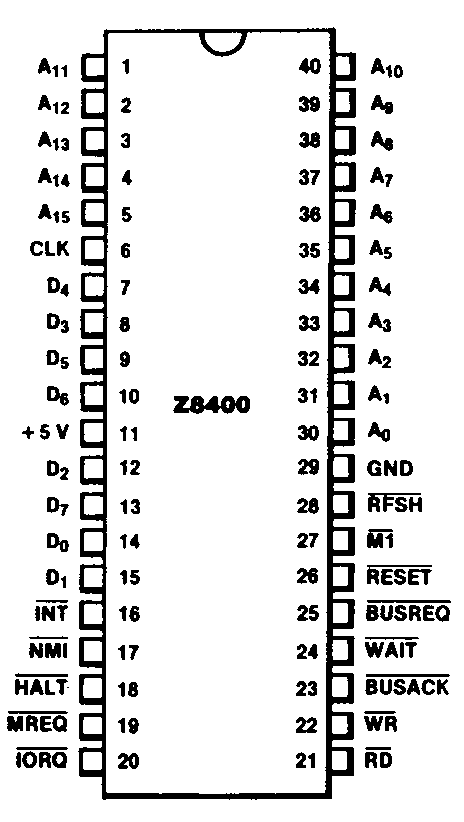
\includegraphics[width=.25\linewidth]{Reischl/img/z80-cpu-pinning-1}}\qquad
    \subfloat{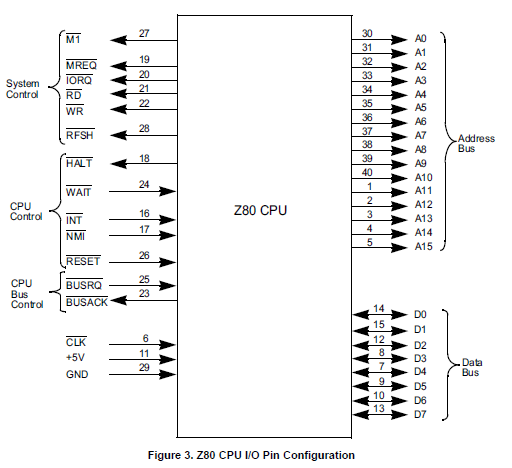
\includegraphics[width=.6\linewidth]{Reischl/img/z80-cpu-pinning-2}}\qquad
    \caption[Z80 CPU Pinning]{CPU Pinning}
    \label{fig:z80-cpu-pinning}
\end{figure}

\subsubsubsection{Funktionsweise und Blockschaltbild}
\fig{z80-cpu-bsb}{Z80 CPU Blockschaltbild}{CPU Blockschaltbild}{\textwidth}{Reischl/img/z80-cpu-bsb}
Die Z80 CPU ist ein 8-Bit-Mikroprozessor, der von Zilog aufbauend auf dem Intel 8080 entwickelt wurde. Der Mikroprozessor basiert auf einer Von-Neumann Architektur und ist als CISC-Maschine (Complex Instruction Set Computer) ausgeführt.

Die Architektur besteht aus Steuerwerk, Registerbank und Recheneinheit. Das Steuerwerk setzt sich aus dem Befehlsregister zum Abspeichern des auszuführenden Befehls, dem Decoder zum Entschlüsseln des in Hex-Code abgespeicherten Befehls und dem Controller Sequencer zum Erzeugen von Steuersignalen zusammen. Die Registerbank besteht aus 6 8-Bit-Universalregistern und speziellen Registern wie Akkumulator, Flagregister, Stackpointer und Program Counter. Die Spiegelung der Universalregister wird für bestimmte Befehle wie etwa Interrupts benötigt, wo der Letztstand vor dem Auslösen eines Interrupts nicht extra im Speicher abgelegt werden muss. Die Ausführung der Befehle erfolgt durch die Recheneinheit, deren zentrales Element die ALU, die Arithmetic Logic Unit, bildet.

Die Kommunikation mit der Peripherie erfolgt über einen 16Bit-Adressbus, einen 8Bit breiten Datenbus und den Steuerbus, welcher im obigen Bild als Kontrollbus bezeichnet wird. Der Speicher wird für Programmcode und Daten gleichzeitig genutzt, gleiches gilt für den Datenbus.

Die Programmierung des Z80 erfolgt in einer Assemblersprache. Der Befehlssatz für die Z80 CPU umfasst maximal 256 Befehle, von denen 252 genutzt werden. Die übliche Länge eines Befehls bewegt sich im Bereich von einem bis vier Byte, die Ausführung eines solchen Befehls nimmt eine je nach Art des Befehls im Regelfall einen Zeitraum zwischen einem und 5 Zyklen in Anspruch.

Die verwendete Halbleitertechnologie ist üblicherweise CMOS (Complementary Metal-Oxide Semiconductor) Technologie, ursprünglich wurde NMOS (N-type Metal-Oxide Semiconductor) - und TTL (Transistor-Transistor Logik)-Technologie verwendet. Besitzt der Baustein ein C in seiner Bezeichnung, so handelt es sich um CMOS-Technologie. Alle auf Feldeffekttransistoren basierenden Baugruppen sind TTL-kompatibel.

\subsubsection{CE-Logik}
\fig{z80-ce-bsb}{Z80 CE-Logik Blockschaltbild}{CE-Logik - 74LS244 Decoder Blockschaltbild}{0.5\textwidth}{Reischl/img/z80-ce-bsb}
Die CE-Logik besteht aus 2 Demultiplexern, einem für die Peripherie und einem für das Speicherwerk. Jeder dieser Demultiplexer oder Decoder besitzt 4 Ausgänge, welche für das Enablen der einzelnen Bausteine, also das Aktivieren des jeweiligen CS- bzw. CE-Eingangs, zuständig ist. Die beiden Decoder bilden einen gemeinsamen IC, bei welchem es sich um einen Standard-IC vom Typ 74LS139 handelt.

Der Decoder für den Speicher ermittelt anhand des 16. Bits des Adressbusses, ob der EPROM oder der SRAM ausgewählt wird. Da nur 2 der 4 Ausgänge verwendet werden, wird der Eingang 1A1 permanent gegen Masse gelegt, der Eingang 1A0 wird mit der Leitung A15, dem 16. Bit des Adressbusses, verbunden. Ist das 16. Bit 1, wird der SRAM enabled, bei 0 der EPROM. Wie der Wahrheitstabelle zu entnehmen ist, wird der jeweilige Chip erst enabled, wenn am Enable-Eingang des Multiplexers ein Low-Pegel anliegt. Dieser Eingang ist im Fall der CE-Logik für EPROM und SRAM mit dem Memory Request (MREQ) belegt.

Der zweite Decoder ist für die Peripherie zuständig Anhand des 7. und 8. Bits des Adressbusses wird bei 00 der CTC, bei 01 der SIO, bei 10 der PIO und bei 11 der DMA Controller aktiviert. Hier gilt wiederum, dass der Decoder für die Peripherie erstdurch den I/O Request enabled werden muss.

Anmerkung: Da alle ein- und Ausgänge des Datenbusses invertiert sind, handelt es sich bei logisch 1 um einen Low-Pegel und bei logisch 0 um einen High-Pegel.
\tabpdf{z80-ce-wahrheit}{Z80 Wahrheitstabelle Demultiplexer}{Wahrheitstabelle Demultiplexer}{0.75\textwidth}{Reischl/img/z80-ce-wahr}

\subsubsection{PIO -- Parallel Input/Output Controller}
\subsubsubsection{Pinning}
\begin{figure}[H]
    \subfloat{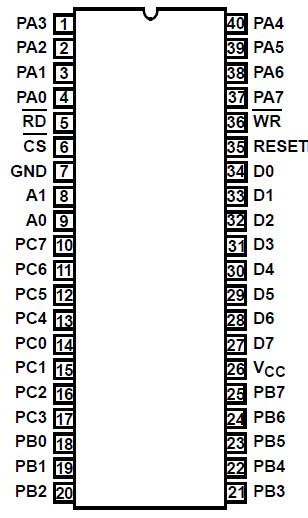
\includegraphics[width=.25\linewidth]{Reischl/img/z80-pio-pinning-1}}\qquad
    \subfloat{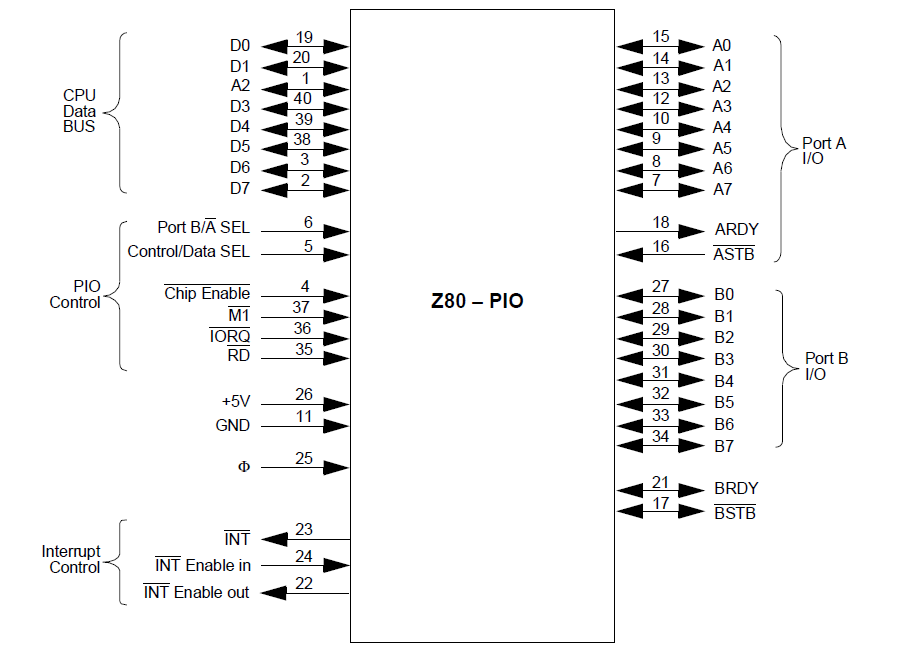
\includegraphics[width=.6\linewidth]{Reischl/img/z80-pio-pinning-2}}\qquad
    \caption[Z80 PIO Pinning]{8255 PIO Pinning \cite{z80:pio}}
    \label{fig:z80-pio-pinning}
\end{figure}

\subsubsubsection{Blockschaltbild und Funktionsbeschreibung}
\fig{z80-pio-bsb}{Z80 PIO Blockschaltbild}{8255 PIO Blockschaltbild \cite{z80:pio}}{\textwidth}{Reischl/img/z80-pio-bsb}
Der 82C55 ist ein von Intel entwickelter Interface-Baustein, welcher als paralleler I/O Port fungiert, deshalb die Bezeichnung PIO. Als solcher bildet er die Schnittstelle zwischen Ein- oder Ausgabeeinheit und Datenbus. Der PIO besitzt 3 Ports zu je 8 Portleitungen, wodurch insgesamt 24 Ein-/Ausgänge eingesetzt werden können. Jeder der 3 Ports besitzt ein Portregister, die jeweils über eine eigene Adresse verfügen.
Alle 3 Ports können einzeln konfiguriert werden, als Eingang oder als Ausgang. Die Konfiguration der einzelnen Ports erfolgt über das Control Register des PIO, welches ebenfalls über eine eigene Adresse verfügt.
\subsubsubsection{Konfiguration des PIO}
Der Port B des Parallel Input/Output Controllers soll als Output für die Ausgabe über LED konfiguriert werden, Port A als Input für das Einlesen der Schalterstellungen des DIL-Schalters. Die Konfiguration erfolgt durch Senden der Konfiguration an die Adresse des Steuerregisters.
\fig{z80-pio-konf}{Z80 Konfiguration PIO}{Konfiguration PIO 8255 \cite{z80:pio}}{0.5\textwidth}{Reischl/img/z80-pio-konf}

\subsubsection{SIO -- Serial Input/Output Controller}
\subsubsubsection{Pinbelegung}
\begin{figure}[H]
    \subfloat{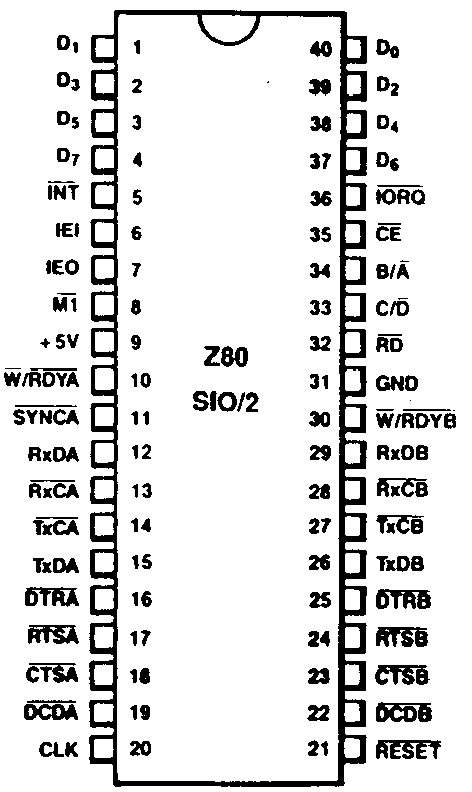
\includegraphics[width=.25\linewidth]{Reischl/img/z80-sio-pinning-1}}\qquad
    \subfloat{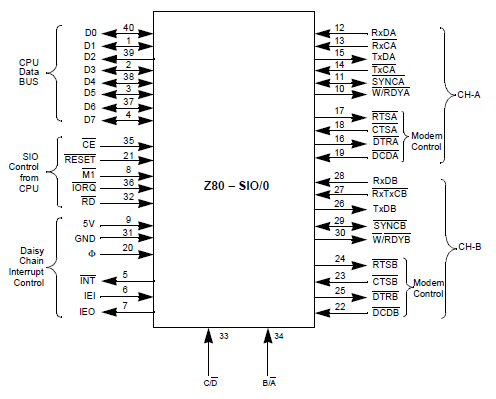
\includegraphics[width=.6\linewidth]{Reischl/img/z80-sio-pinning-2}}\qquad
    \caption[Z80 SIO Pinning]{SIO Pinning \cite{z80:sio}}
    \label{fig:z80-sio-pinning}
\end{figure}

\subsubsubsection{Blockschaltbild und Funktionsbeschreibung}
\fig{z80-sio-bsb}{Z80 SIO Blockschaltbild}{SIO Blockschaltbild \cite{z80:sio}}{\textwidth}{Reischl/img/z80-sio-bsb}
Der SIO dient dazu, dass die Z80 CPU über serielle Schnittstellen Daten austauschen kann. Der Baustein wurde von Zilog entwickelt und trägt die Bezeichnung Z84C40, das verwendete Modell Z84C4006. Der Serial Input/Output Controller verfügt über 2 Kanäle, es können also bis zu 2 serielle Schnittstellen genutzt werden. Als Seriell/Parallel-Parallel/Seriell Konverter kann der SIO synchrone als auch asynchrone Protokolle verarbeiten. Weiters besitzt der SIO die Fähigkeit, Interrupts auszulösen.

Adressiert werden kann beim SIO nur für jeden Kanal ein Daten- und ein Steuerregister (Cannel A/B Data/Control Register).

\subsubsubsection{Konfiguration}
Da die Konfiguration des SIO recht umfangreich ist und somit den Rahmen der Dokumentation sprengen würde, muss an dieser Stelle auf die vorgegebene Konfiguration in den Beispielprogrammen und auf das Z80 Peripherals User Manual verwiesen werden.

Write Register:
\begin{itemize}
    \item WR0: Register pointers, CRC initialize, initialization commands for the various modes and more
    \item WR1: Transmit/Receive interrupt and data transfer mode definition
    \item WR2: Interrupt vector (Channel B only)
    \item WR3: Receive parameters and controls
    \item WR4: Transmit/Receive miscellaneous parameters and modes
    \item WR5: Transmit parameters and controls
    \item WR6: Sync character or SDLC address field
    \item WR7: Sync character or SDLC flag
\end{itemize}

Read Register:

\begin{itemize}
    \item RR0: Transmit/Receive buffer status, interrupt status, and external status
    \item RR1: Special Receive Condition status
    \item RR2: Modified interrupt vector (Channel B only)
\end{itemize}

Die im Programm SIO V24 Echo vorgenommene Konfiguration für den SIO:

\begin{itemize}
    \item Baudrate: 9600 Baud/sek
    \item Stoppbits: 1
    \item Startbits: 1
    \item Wortlänge: 8 Bit
    \item Paritätsbits: keines
\end{itemize}

\subsubsection{Einbindung der Ein- und Ausgabeeinheiten (SIO, PIO)}
\begin{figure}[H]
    \centering
    \subfloat{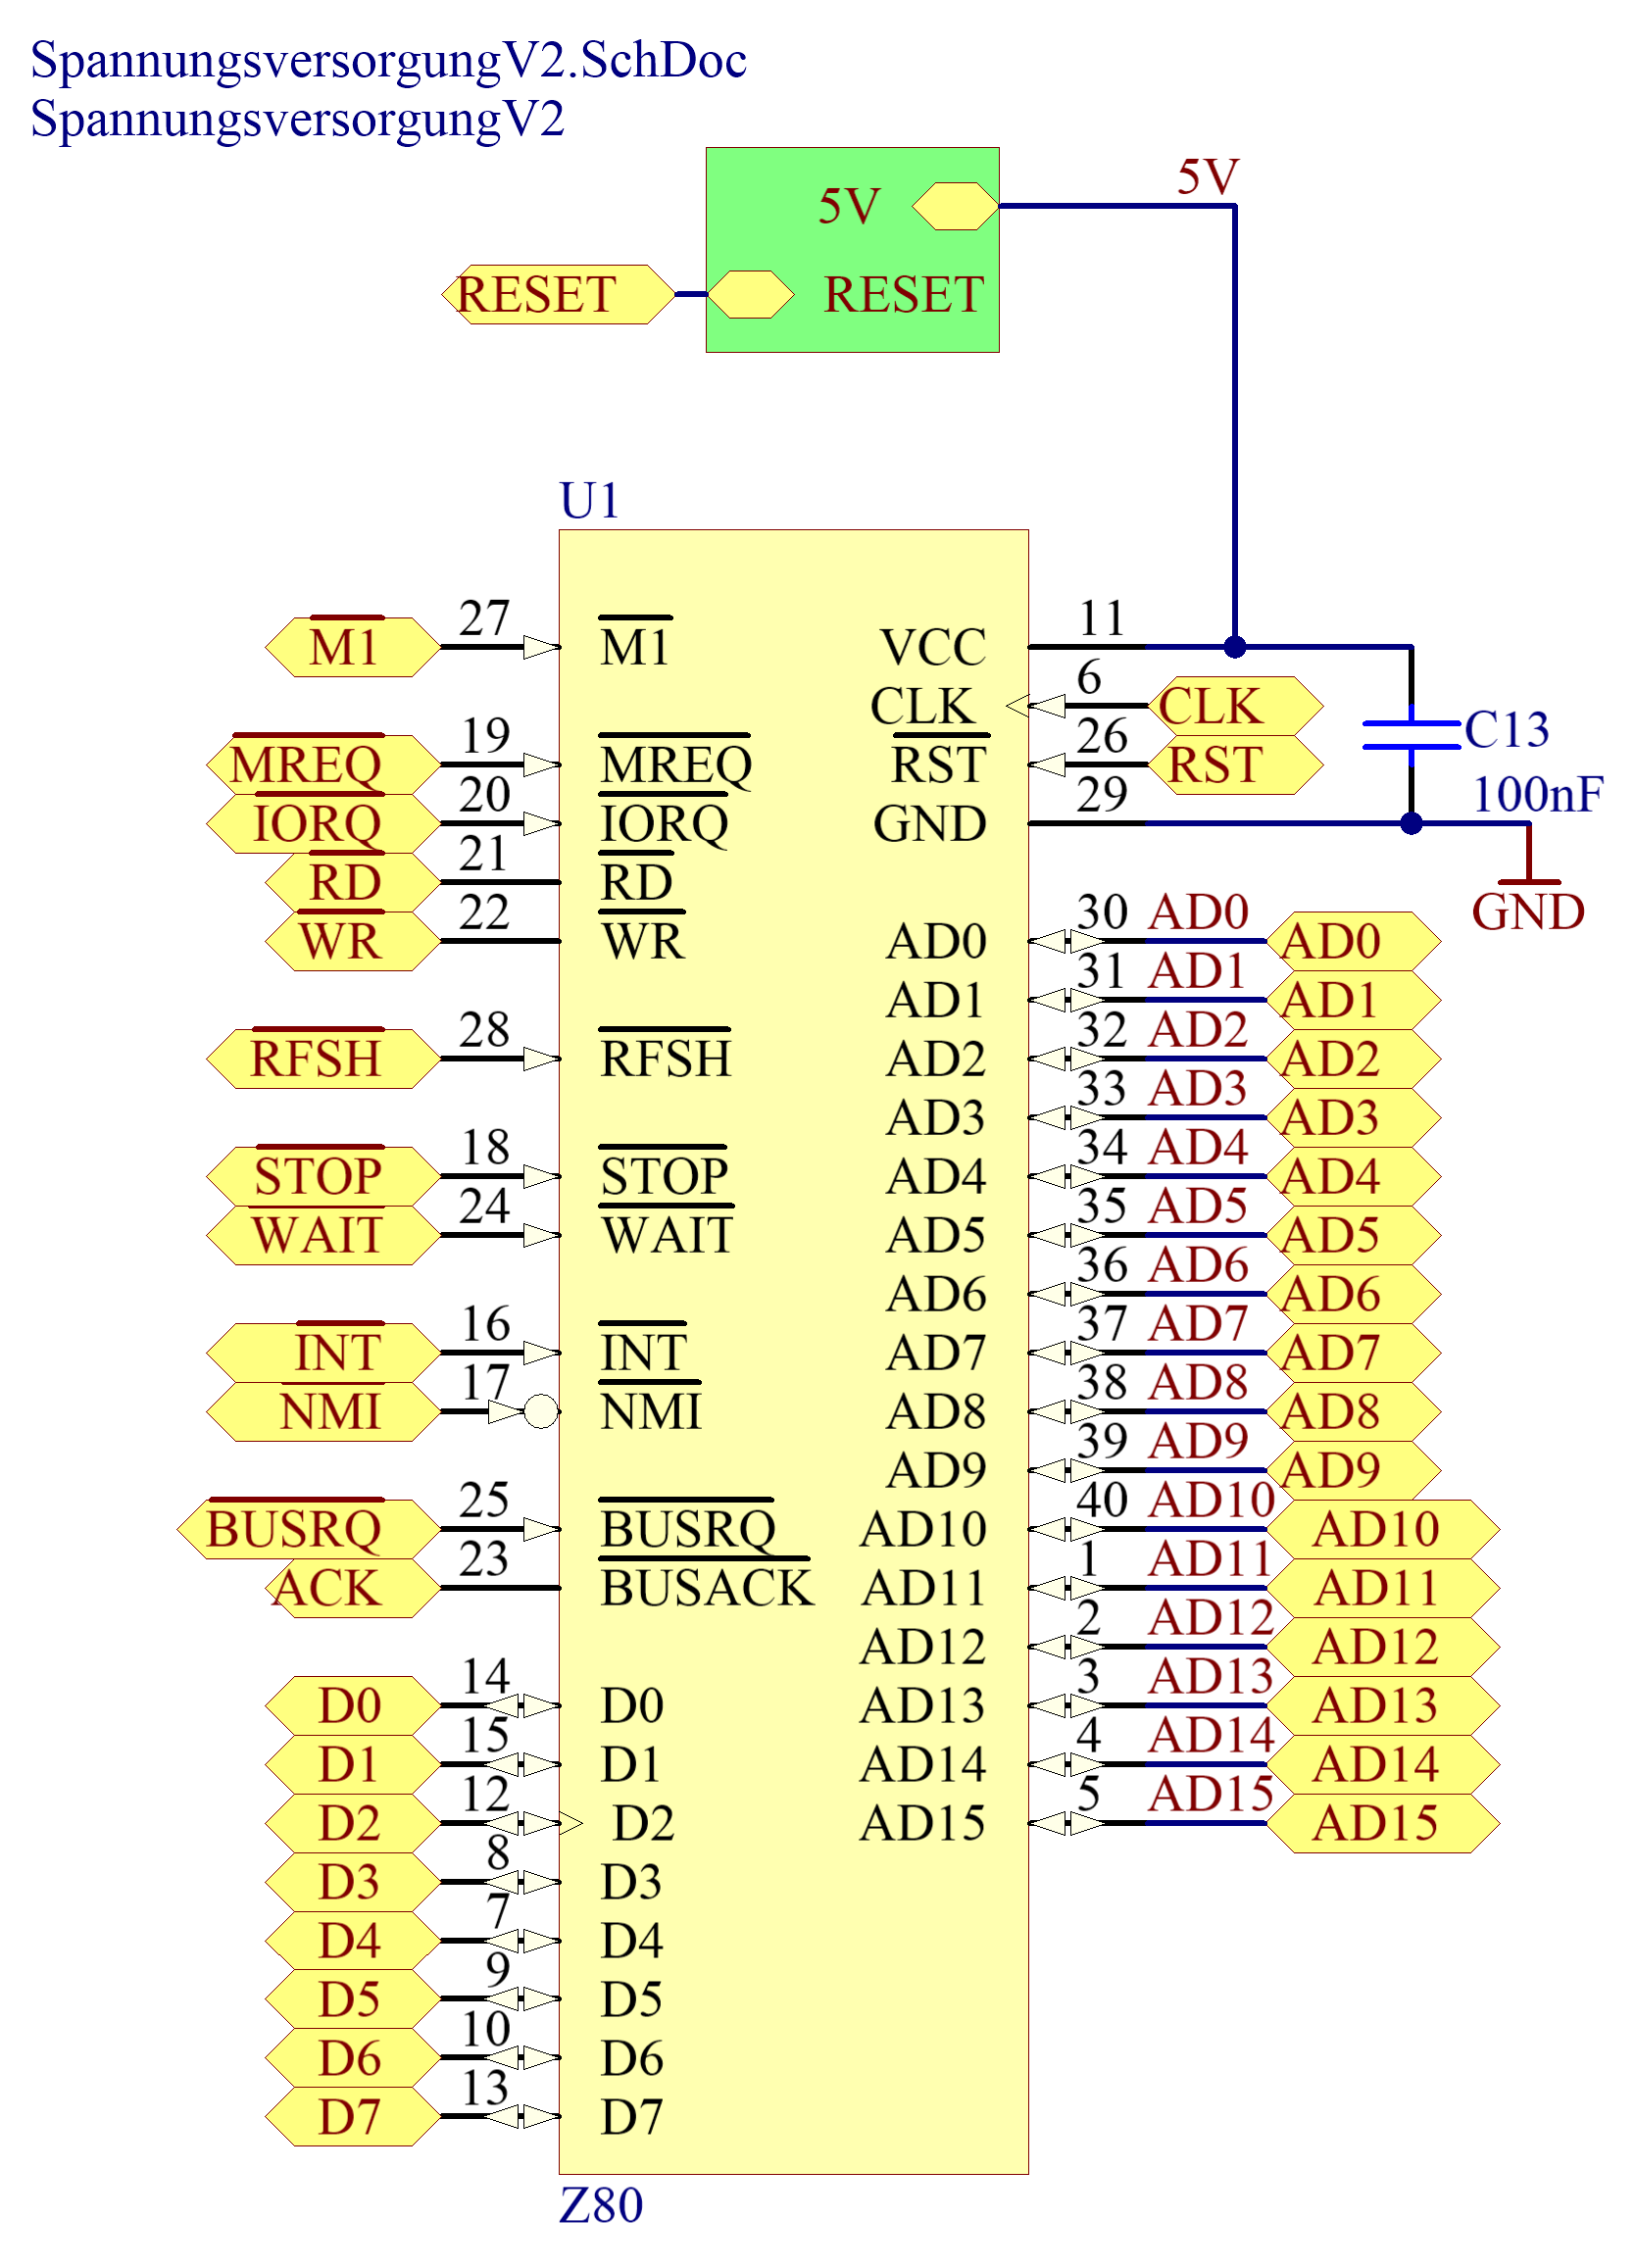
\includegraphics[width=.4\linewidth]{Reischl/img/z80-io-1}}\qquad
    \subfloat{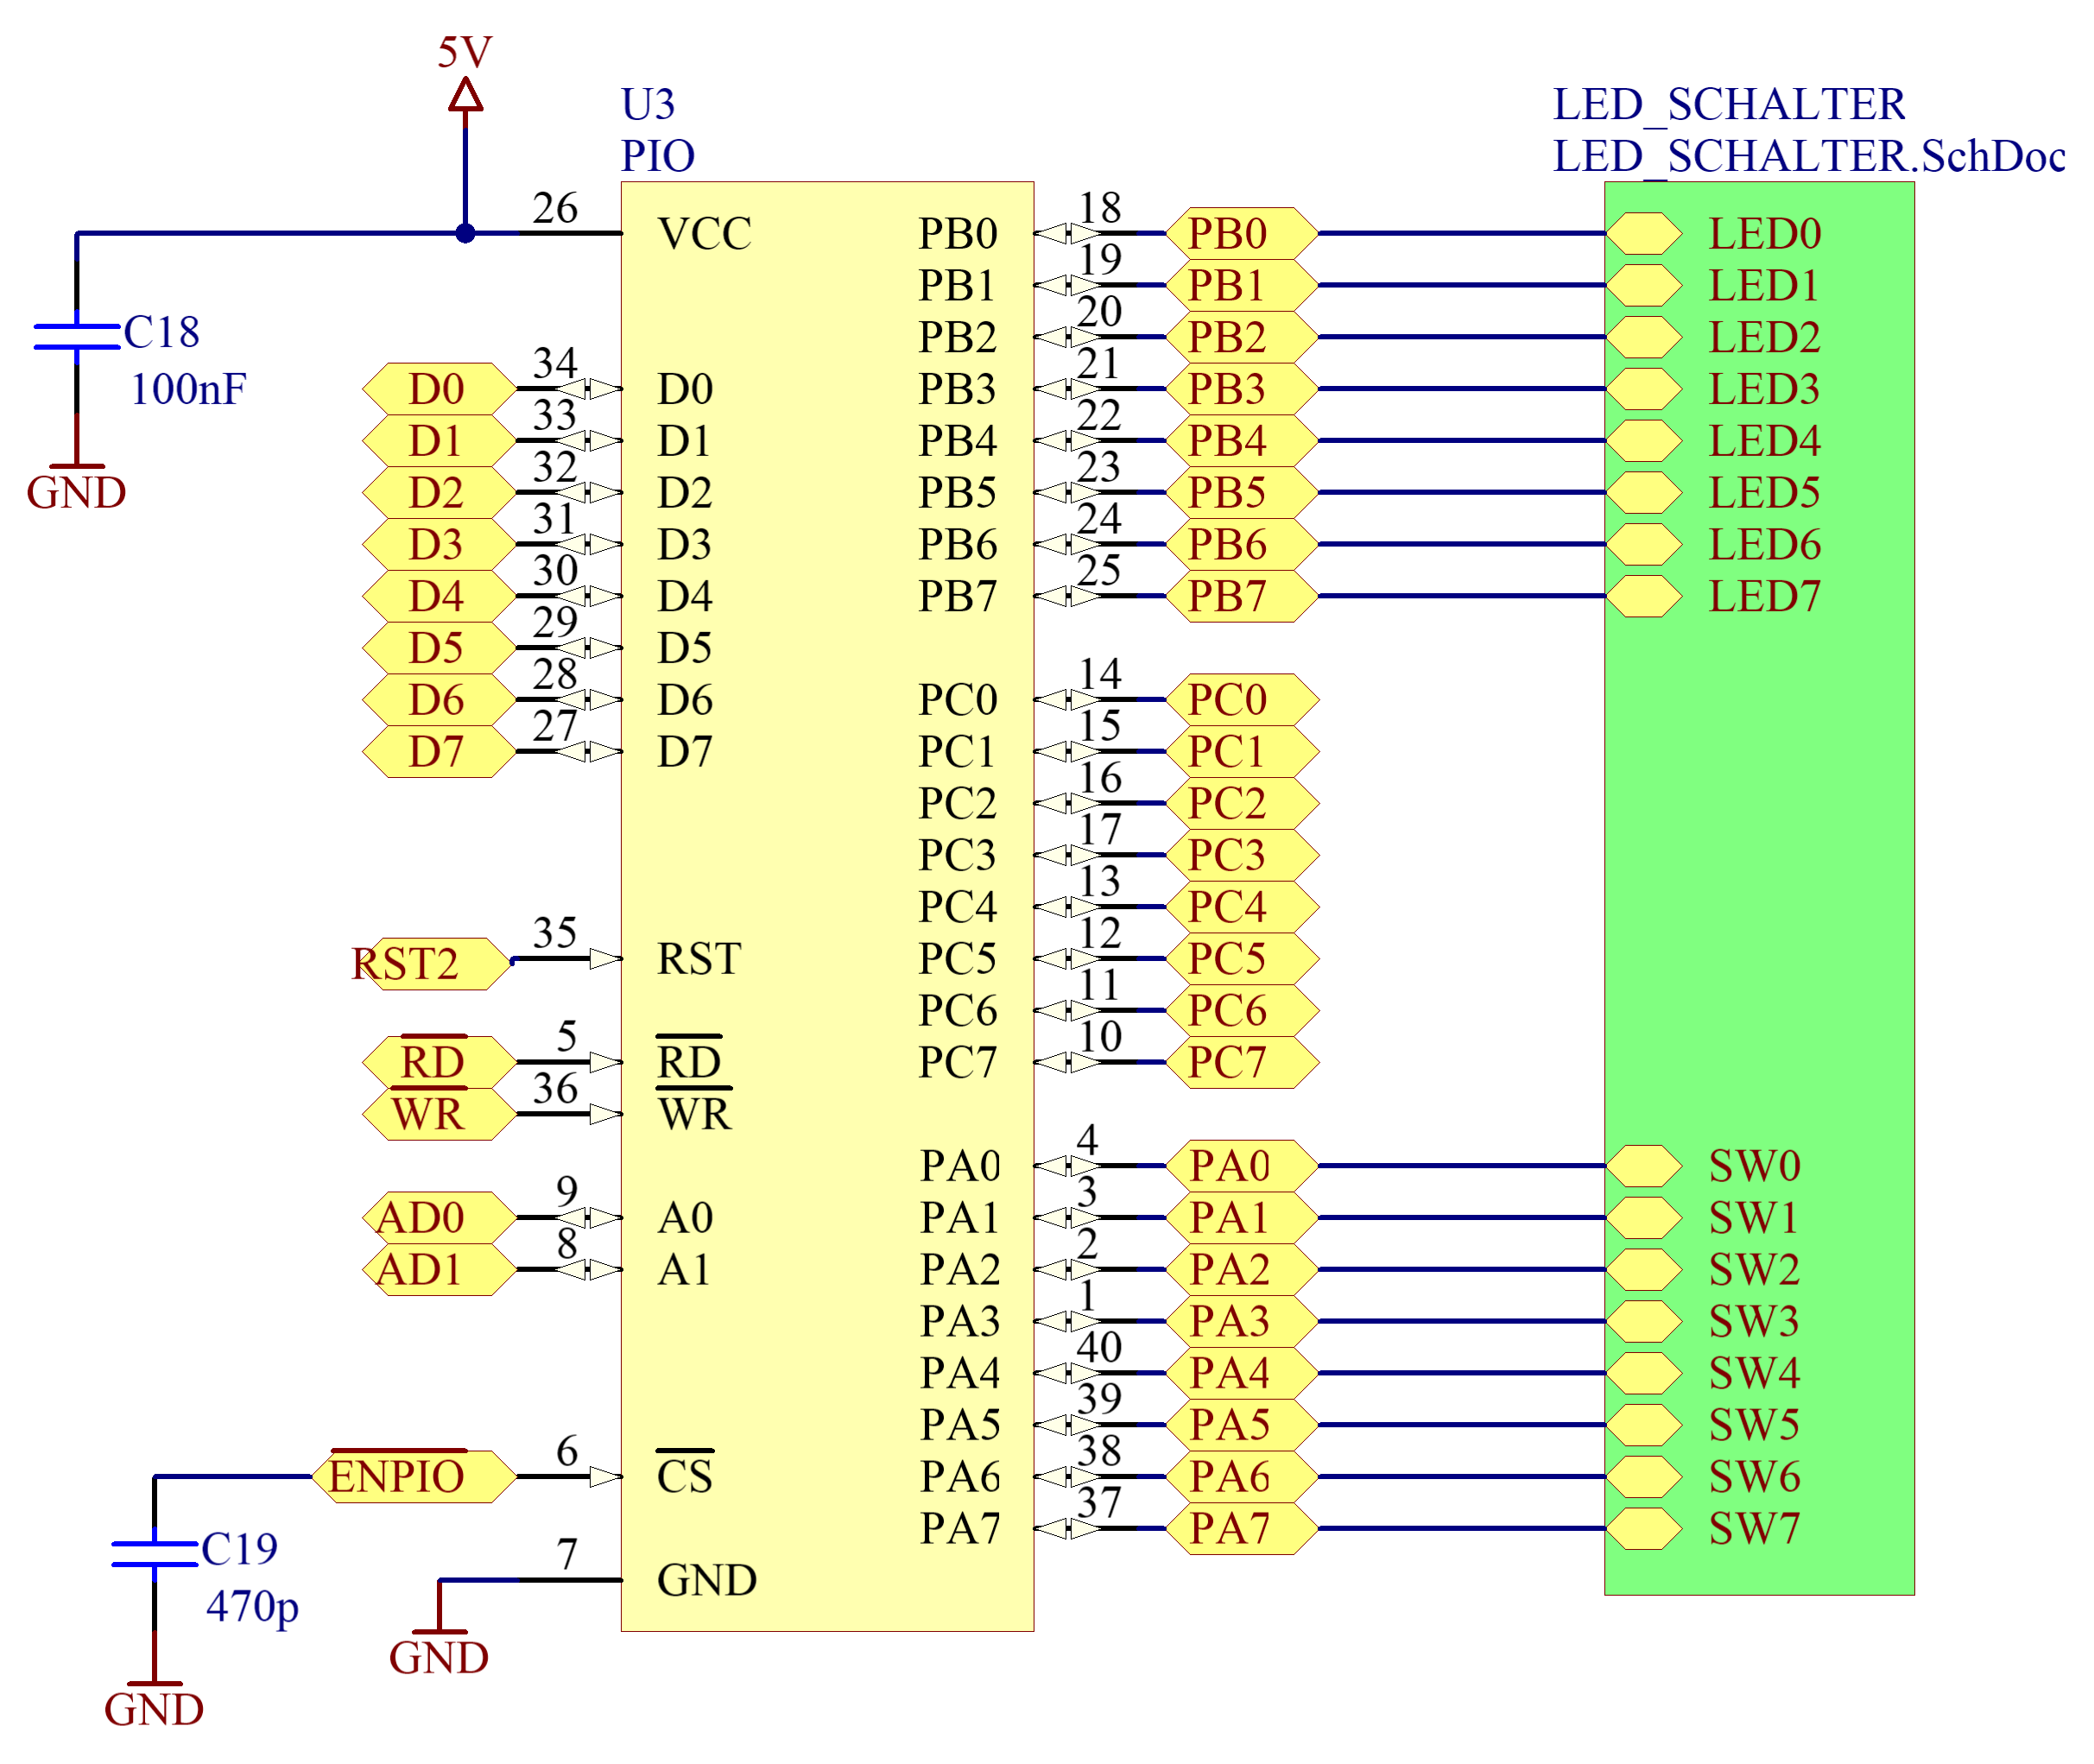
\includegraphics[width=.4\linewidth]{Reischl/img/z80-io-2}}\qquad
    \subfloat{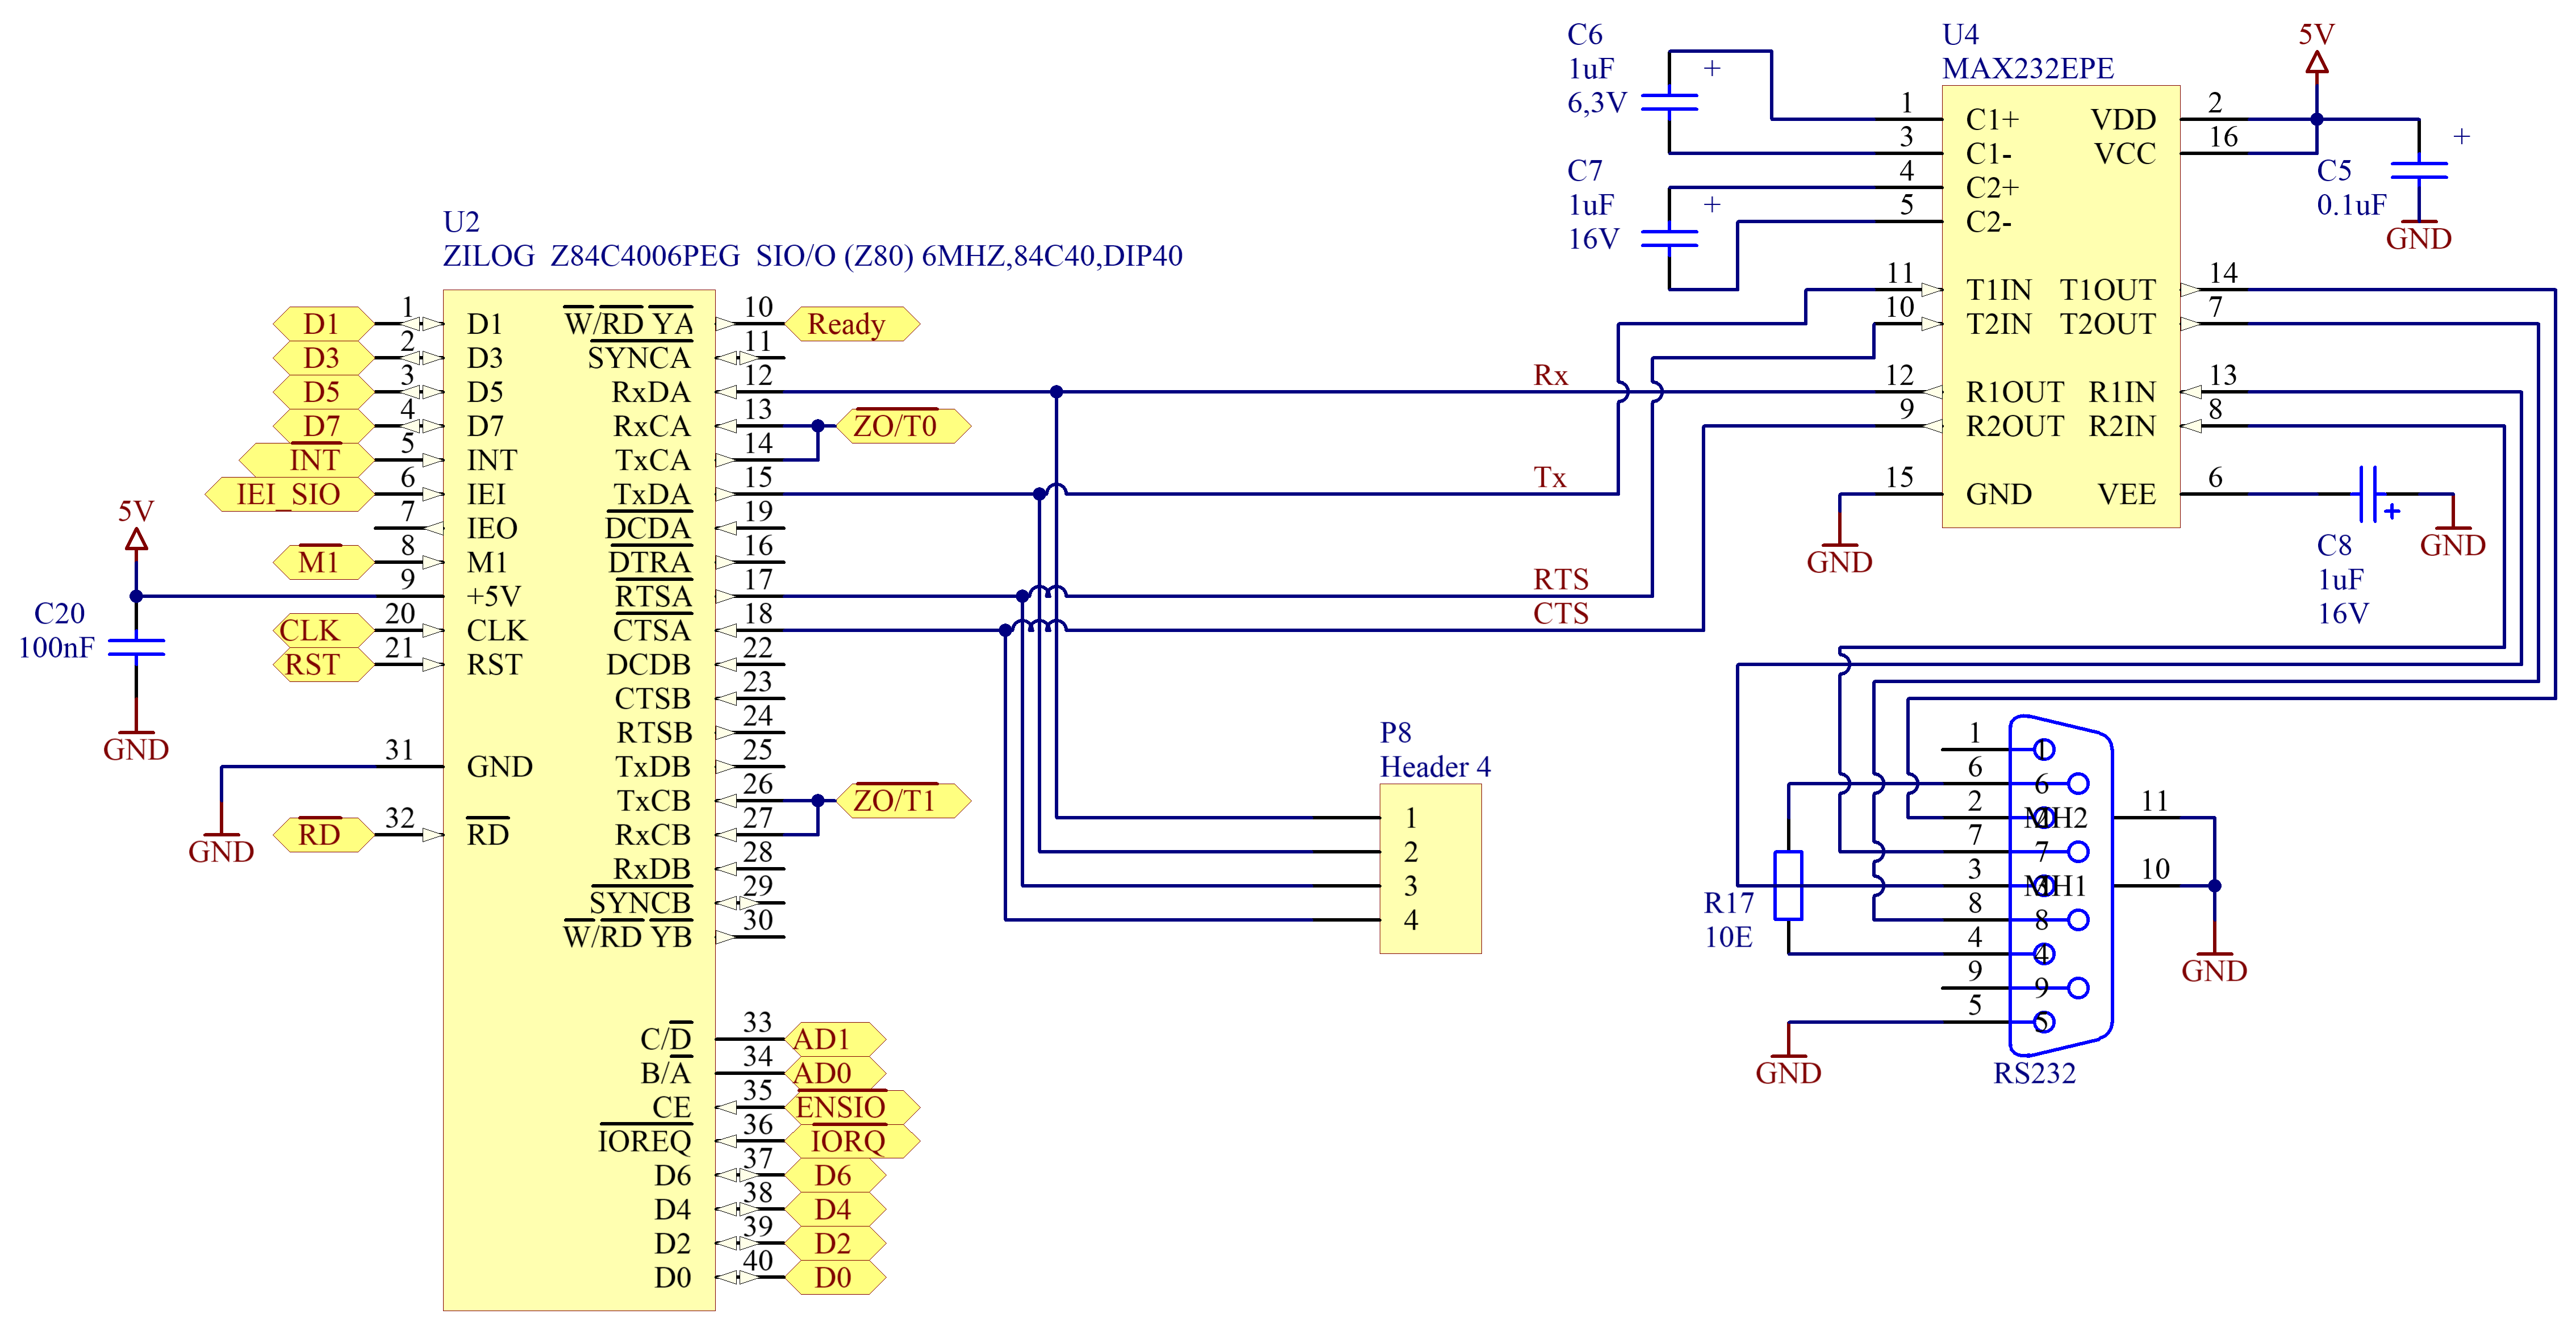
\includegraphics[width=\linewidth]{Reischl/img/z80-io-3}}\qquad
    \caption[Z80 Ein-/Ausgabeeinheiten]{Ein- und Ausgabeeinheiten}
    \label{fig:z80-io}
\end{figure}
Zur Kommunikation mit der Außenwelt besitzt das Z80 Minimalsystem einen 8-fach DIL-Schalter und ein 8-fach LED-Array sowie eine serielle Schnittstelle (RS232) für den Datenaustausch mit einem PC oder einem Terminal.

Der 8-fach Schalter und das LED-Array sind über den PIO Baustein 8255 mit der CPU verbunden, die serielle Schnittstelle wird über den Z80 SIO Baustein realisiert. Die 8 Schalter sind am Port 8 des PIO angeschlossen, das LED-Array ist mit dem Port B verbunden. Der SIO nutzt den Port A für die serielle Schnittstelle. Da der SIO nur TTL-Pegel liefert, wird ein Pegelwandler vom Typ MAX232 für die Umwandlung in RS232-Pegel eingesetzt.

Beide ICs sind über den 8 Bit breiten Datenbus und dem Low Byte des Adressbusses mit der CPU verbunden. Die die Datenflusssteuerung erfolgt über die Signale RD und WR. Beide Bausteine besitzen intern 4 adressierbare Register. Mithilfe dieser Register wird die Konfiguration und der Datenaustausch mit der CPU durchgeführt.

Die ICs selbst besitzen nur jeweils 2 Adressleitungen, A0 und A1. Das 7. und 8. Bit des Adressbusses nutzt die CE-Logik zum Enablen der Peripherieeinheiten. A3 bis A5 bleiben bei der Kommunikation mit der Peripherie ungenutzt ebenso wie das gesamte High Byte des Adressbusses.

Für den PIO lauten die Adressen der Portregister 80 für Port A, 81 für Port B und 82 für Port C. Das Konfigurationsregister besitzt die Adresse 83.

Der SIO nutzt den Datenbus dafür, um zu übermitteln, welcher Port (AD0: 0=A; 1=B) angesprochen wird und ob konfiguriert wird (AD1=1) oder ob Daten übertragen werden (AD1=0). Bei der Anwendung mit dem Z80 Minimalsystem besitzt das Datenregister des Kanals A die Adresse 40, das Datenregister des Kanals B die Adresse 41, das Steuerregister des Kanals A die Adresse 42 und das Steuerregister des Kanals B die Adresse 43. M1, also die Leitung, welche einen Machine Cycle One und damit einen Instruction Fetch kennzeichnet, bewirkt gemeinsam mit einem I/O Request einen Interrupt, wenn über die Daisy Chain (IEI) der SIO die höchste Priorität erhält.

\subsubsection{CTC -- Counter Timer Circuit}
\subsubsubsection{Pinning}
\begin{figure}[H]
    \subfloat{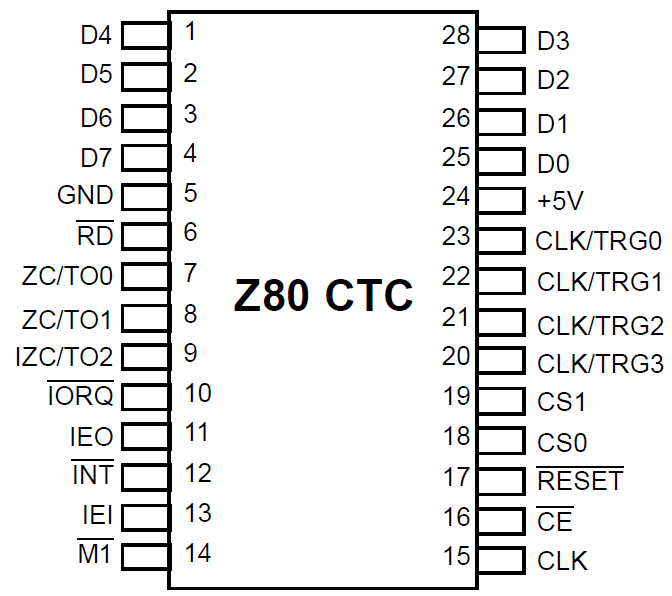
\includegraphics[width=.4\linewidth]{Reischl/img/z80-ctc-pinning-1}}\qquad
    \subfloat{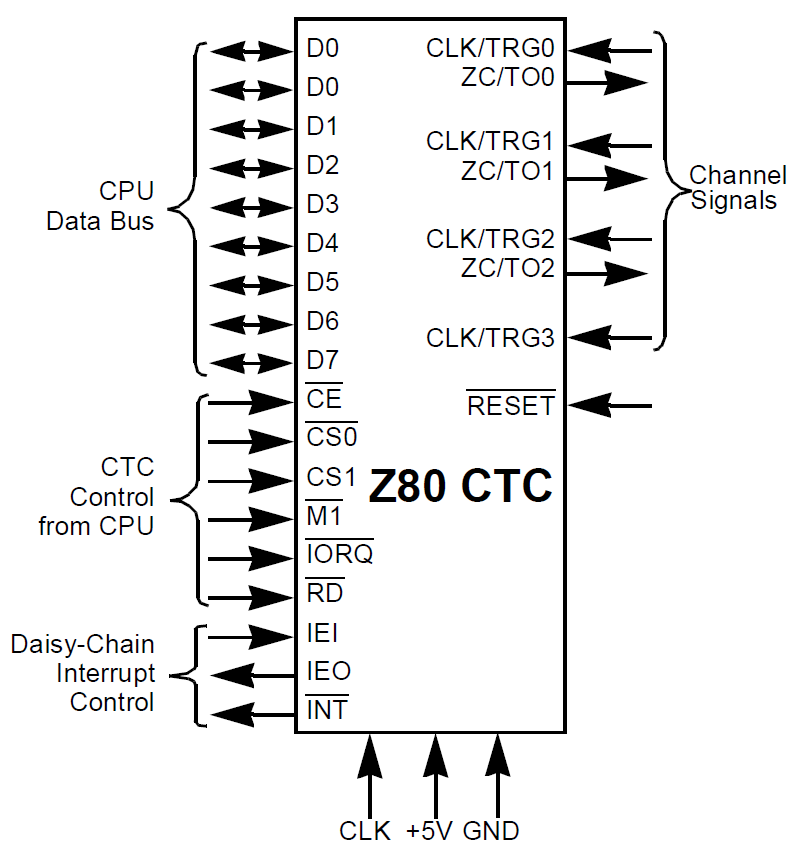
\includegraphics[width=.4\linewidth]{Reischl/img/z80-ctc-pinning-2}}\qquad
    \caption[Z80 CTC Pinning]{CTC Pinning \cite{z80:ctc}}
    \label{fig:z80-ctc-pinning}
\end{figure}

\subsubsubsection{Blockschaltbild und Funktionsbeschreibung}
\fig{z80-ctc-bsb}{Z80 CTC Blockschaltbild}{CTC Blockschaltbild \cite{z80:ctc}}{\textwidth}{Reischl/img/z80-ctc-bsb}
Beim Counter Timer Circuit handelt es sich um einen Baustein für die Steuerung von zeitabhängigen Vorgängen. Der Z80 CTC trägt die generelle Bezeichnung Z84C30, der verwendete IC heißt 84C3006PEG. Der CTC stellt grundsätzlich 3 verschiedene Funktionen bereit, nämlich den Betrieb als Zähler, als Counter und die Fähigkeit, Interrupts auszulösen. Intern verfügt der Counter Timer Circuit über insgesamt 4 voneinander unabhängige Kanäle. Jeder Kanal besteht aus einem Zähler, der als Zähler und als Time betrieben werden kann. Für die Konfiguration und die Steuerung der internen Abläufe ist die Steuerlogik zuständig, das Interrupt Handling und das Erzeugen solcher wird durch die Interrupt Logik vorgenommen.

Als Zähler arbeitet das System synchron mit dem Systemtakt. Die höchstmögliche Zählfrequenz entspricht der Frequenz des Systemtaktes. Der Zähler ist ein Downcounter wird 0 erreicht, wird je nach Konfiguration der Inhalt des Zeitkonstantenregisters (Time Constant Register, siehe Aufbau eines CTC-Kanals) neu geladen und ein Interrupt ausgelöst. So wie der Zähler neben dem Systemtakt auch Ereignisse am Pin TRGx des jeweiligen Kanals zählen kann, kann auch im Timerbetrieb dieser Eingang genutzt werden, um den Timer zu starten. Auf das Signal am Pin TRGx des jeweiligen Kanals wird also getriggert. Der Timer zählt die Impulse des Systemtakts nach dem Prescaler, der den Takt entweder um den Faktor 16 oder 256 teilt. Beim Nulldurchgang des Zählers wird der Downcounter des Timers aus dem Zeitkonstantenregister neu geladen, ein Signal am Pin ZC/TOx des jeweiligen Kanals erzeugt und bei Bedarf ein Interrupt generiert.

\fig{z80-ctc-kan}{Z80 CTC Kanal}{Aufbau eines CTC-Kanals \cite{z80:ctc}}{0.75\textwidth}{Reischl/img/z80-ctc-kan}

\subsubsubsection{Konfiguration des CTC}
Ansteuerung der Kanäle über den Adressbus (AD0=CS0, DA1=CS1):
\tabpdf{z80-ctc-konfig}{Z80 Belegung CTC Kanäle}{Belegung CTC Kanäle \cite{z80:ctc}}{0.75\textwidth}{Reischl/img/z80-ctc-konfig}
Die Konfiguration wird ähnlich wie beim PIO durch Adressierung des Steuerregisters vorgenommen, allerdings besitzt jeder Kanal ein eigenes Steuerregister (Control Register), weshalb die Konfiguration für jeden Kanal einzeln vorgenommen wird. Weiters besitzt jeder Kanal ein Zeitkonstantenregister und ein Interruptvektorregister. Die Konfiguration aller 3 Register erfolgt immer mit derselben Adresse, da die Daten intern im CTC in das richtige Register weitergeschoben werden. Deshalb ist es wichtig, die Reihenfolge der Konfiguration einzuhalten und alle 3 Register zu konfigurieren.
\tabpdf{z80-ctc-konfig-2}{Z80 CTC Channel Control Register Teil 1}{CTC Channel Control Register Teil 1 \cite{z80:ctc}}{\textwidth}{Reischl/img/z80-ctc-konfig-2}
\tabpdf{z80-ctc-konfig-3}{Z80 CTC Channel Control Register Teil 2}{CTC Channel Control Register Teil 2 \cite{z80:ctc}}{\textwidth}{Reischl/img/z80-ctc-konfig-3}
\tabpdf{z80-ctc-konfig-4}{Z80 CTC Zeitkonstentenregister}{CTC Zeitkonstantenregister \cite{z80:ctc}}{\textwidth}{Reischl/img/z80-ctc-konfig-4}
\tabpdf{z80-ctc-konfig-5}{Z80 CTC Interrupt Vector Register und Konfiguration}{CTC Interrupt Vector Register und Konfiguration \cite{z80:ctc}}{\textwidth}{Reischl/img/z80-ctc-konfig-5}
In dieser Anwendung wird nur der Kanal A konfiguriert:

\begin{itemize}
    \item A5: Enable Interrupt; Timer Mode; Prescaler 256; Trigger: fallende Flanke; Automatischer Trigger, wenn die Zeitkonstante geladen wird; Zeitkonstante wird ebenfalls geladen; kein Software-Reset; Control\\
    \item FF: Zeitkonstante = 256
    \item A8: Kanal 0, Interrupt Vektor (Zum Auslösen eines Interrupts)
\end{itemize}

\subsubsubsection{Verbindung des Timerbausteins mit der CPU}
\fig{z80-zeit}{Z80 Zeitabhängige Vorgänge}{Zeitabhängige Vorgänge}{\textwidth}{Reischl/img/z80-zeit}
Der Counter-Timer-Circuit kann sowohl als Timer als auch als Zähler eingesetzt werden. Er besitzt 3 Kanäle, von denen jeder über einen Timer verfügt. Dieser Timer kann sowol als Timer als auch als Zähler genutzt werden. Jeder Kanal einen Eingang CKT/TRGx auf den getriggert werden kann. Im Timer Mode kann der Timer durch diesen Triggereingang gestartet werden und im Counter Mode können dort auftretende Imulse gezählt werden. Jeder Kanal besitzt ein 3 Byte großes Schieberegister zur Konfiguration, welches über die Adressleitungen A0 und A1 adressiert werden kann. Die Adressen für das Z80 Minimalsystem lauten 00 für den Kanal 1 bis 03 für den Kanal 4. als Eingang für den Zähler oder Start für den Timer genutzt werden kann.

\subsubsection{EEPROM -- Erasable Programmable ReadOnly Memory}
\subsubsubsection{Pinning}
\fig{z80-eprom-pinning}{Z80 EEPROM Pinning}{EEPROM Pinning \cite{z80:eprom}}{0.3\textwidth}{Reischl/img/z80-eprom-pinning}

\subsubsubsection{Funktionsweise}
\fig{z80-eprom-cell}{Z80 Aufbau einer Speicherzelle}{Aufbau einer Speicherzelle \cite{z80:eprom}}{0.4\textwidth}{Reischl/img/z80-eprom-cell}
Beim EPROM handelt es sich um einen 32kiB großen NMOS EPROM, welcher beim Z80 Minimalsystem als Programm- und Datenspeicher dient und von diversen Herstellern wie etwa ST Microelectronics, NEC oder Intel gefertigt wurde bzw. immer noch wird. Organisiert ist der 27256 EPROM als 32k *8 Bit Speicher, es können also 32768 Wörter zu je 8 Bit über den 15 Bit breiten Adressbus und den Steuerbus angesprochen und über den 8-Bit-Datenbus abgerufen werden. Beschrieben kann der EPROM von der CPU nicht werden. Die Programmierung des EPROM erfolgt nicht in der Schaltung, sondern dieser muss aus der Schaltung entfernt werden und mit einem eigenen Programmiergerät beschrieben werden.

\subsubsection{SRAM -- Static Random Access Memory}
\subsubsubsection{Pinning}
\fig{z80-sram-pinning}{Z80 SRAM Pinning}{62256 SRAM Pinning \cite{z80:ram}}{0.4\textwidth}{Reischl/img/z80-sram-pinning}

\subsubsubsection{Funktionsbeschreibung und Blockschaltbild}
\fig{z80-sram-bsb}{Z80 SRAM Blockschaltbild}{62256 SRAM Blockschaltbild \cite{z80:ram}}{0.5\textwidth}{Reischl/img/z80-sram-bsb}
Der SRAM ist ebenfalls wie der EPROM 32kiB groß und als 32k x 8 Bit Speicher organisiert. Da der RAM im Gegensatz zum EPROM während des Betriebes des Minimalsystems auch beschrieben werden kann, wird anhand von WE und OE entschieden, ob Daten gelesen oder gespeichert werden. Dabei muss der Chip immer über CE enabled sein. Wie dem obigen Blockschaltbild zu entnehmen ist, kann immer nur der Dateneingang oder der Datenausgang aktiv sein.

\subsubsection{Verbindung des Speichers mit der CPU}
\fig{z80-speicher}{Z80 Speicheraufbau}{Speicheraufbau}{\textwidth}{Reischl/img/z80-speicher}
Die Speicher (32kx 8 EPROM und 32k x 8 SRAM) sind in erster Linie über den Daten- und den Adressbus mit der CPU verbunden. Die byteweise Adressierung der Speicherzellen erfolgt über 15 der 16 Bit des Adressbusses (AD0 bis AD14), das 16. Bit (AD15) wird von der Chip-Enable-Logik verwendet. Liegt am Eingang des CE-Decoders 0 in Kombination mit einem Memory Request (MREQ) an, wird der CE-Eingang des EPROMS aktiviert, bei 1 wird vom Decoder der CE-Eingang des SRAMs (SRAMEN bzw. CE) aktiv. Wie im Timing ersichtlich ist Verbindung mit dem Datenbus aber erst dann vorhanden, wenn die CPU ein READ (RD) für einen Lesevorgang oder ein WRITE (WR) für einen Schreibvorgang erzeugt. Diese Signale bewirken ein Output Enalbe bzw. ein Write Enable.
\fig{z80-eprom-timing}{Z80 EPROM Timing}{EPROM Timing}{\textwidth}{Reischl/img/z80-eprom-timing}

\subsubsection{DMA-Controller -- Direct Memory Access Controller}
\subsubsubsection{Pinning}
\begin{figure}[H]
    \subfloat{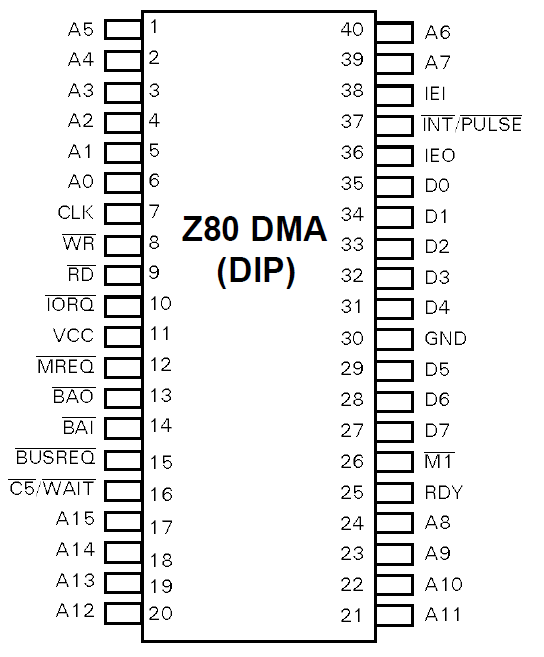
\includegraphics[width=.4\linewidth]{Reischl/img/z80-dma-pinning-1}}\qquad
    \subfloat{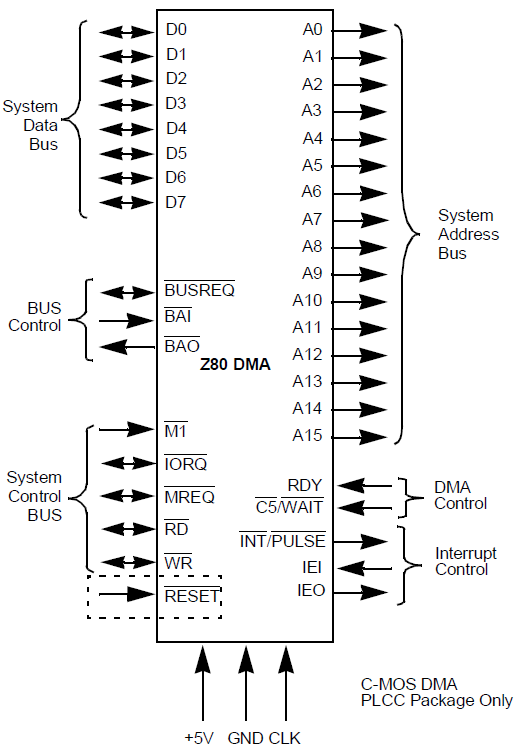
\includegraphics[width=.4\linewidth]{Reischl/img/z80-dma-pinning-2}}\qquad
    \caption[Z80 DMA Pinning]{DMA Pinning \cite{z80:dma}}
    \label{fig:z80-dma-pinning}
\end{figure}

\subsubsubsection{Funktionsbeschreibung und Blockschaltbild}
\fig{z80-dma-bsb}{Z80 DMA Blockschaltbild}{DMA Blockschaltbild \cite{z80:dma}}{\textwidth}{Reischl/img/z80-dma-bsb}
Der DMA Controller ist ein für den Z80 und den Z8000 entwickelter IC mit der Bezeichnung Z8410 bzw. Z84C10. Er ermöglicht einen Speicherdirektzugriff, es werden die Daten also nicht mithilfe der CPU aus dem Speicher geholt und dann von der CPU an die entsprechende Peripherieeinheit übermittelt, sondern direkt zwischen dem Speicher und der jeweiligen Peripherieeinheit ausgetauscht. Diese direkte Kommunikation der Peripheriegeräte mit dem Speicher ist performanter als der Datentransfer via CPU, da ein Zwischenspeichern in den Registern der CPU und ein Instruction Fetch bei jedem Transfer wegfällt. Neben dem Datentransfer zwischen den 2 Ports des DMA Controllers existiert auch eine Suchfunktion. Der DMA kann in 3 verschiedenen Modi betrieben werden: Im Byte- oder Single Mode steht nach jedem übertragenen Byte kann die CPU den Datenbus nutzen, im Burst Mode werden solange Daten übertragen, bis die CPU den Übertragungsvorgang beendet und im Continuous Mode wird die Übertragung der Daten entweder durch das Erfüllen der Stopp-Bedingung oder durch das Erreichen des Endes des zu übertragenden Datensatzes beendet.

Da der DMA Controller in keinem momentan existenten Programm für das Z80 Minimalsystem Verwendung findet, wird auf die Konfiguration und den Aufbau nicht näher eingegangen.

\subsubsection{NMI -- Non Maskable Interrupt}
\fig{z80-nmi-bsb}{Z80 NMI Blockschaltbild}{NMI Blockschaltbild}{0.5\textwidth}{Reischl/img/z80-nmi-bsb}
Soll ein NMI, ein nicht maskierbarer Interrupt durch den Anwender ausgelöst werden, so muss dieser den Taster S1 betätigen. Die Leitung NMI, welche mit einem Pull-Up Widerstand versehen ist, ist mit der CPU verbunden und diese löst dann einen Interrupt aus.

\subsubsection{I/O Einheiten}
\subsubsubsection{Ausgabeeinheit}
Der Port A des PIO ist mit einem 8-fach LED-Array als parallele Ausgabeeinheit ausgestattet (siehe Abbildung unten). Um den Ausgang des PIO nicht zu belasten, wird ein 8-fach Bustreiber verwendet, um die LEDs zu versorgen. Dieser Treiber wirkt invertierend und seine Ausgänge sind mit den Eingängen OE1 und OE2 mittels Jumper J3 deaktivierbar. Ist der Jumper J3 so gesetzt, dass die LEDs versorgt werden können, leuchtet auch eine zusätzliche LED (V9). Wird an den Eingang OE Masse angelegt, wird der Treiberbaustein enabled bzw. aktiviert, da es sich um einen invertierten Eingang handelt. Um die Helligkeit der LEDs von der Anzahl der aktivierten LEDs unabhängig zu machen, sind 2 Dioden in Serie zu den 8 LEDs geschaltet. Diese 2 Dioden ersetzen den sonst üblichen Serienwiderstand bei jeder einzelnen LED. Der Grund für 2 Dioden liegt darin, dass bei der Anwendung von einer einzelnen Diode der Strom durch die LEDs zu hoch ist und damit die Helligkeit.
\fig{z80-ioo-bsb}{Z80 Ausgabe LEDs}{Ausgabe LEDs}{\textwidth}{Reischl/img/z80-ioo-bsb}

\subsubsubsection{Eingabeeinheit}
\fig{z80-ioi-bsb}{Z80 Eingabe-Schalter}{Eingabe-Schalter}{0.75\textwidth}{Reischl/img/z80-ioi-bsb}
Die Eingabeeinheit besteht aus einem 8-fach DIP-Schalter, dessen Ausgang mit Pull-Up Widerständen versehen sind. Ist ein Schalter also offen, liegen am Eingang des Port B des PIO 5V an, wird der Schalter geschlossen, wird der Eingang des PIO mit Masse verbunden und am entsprechenden PIN des PIO liegen 0V an. Da alle Ein- und Ausgänge des Datenbusses invertiert sind, interpretiert die CPU einen offenen Schalter a ls logisch 0 und einen geschlossenen Schalter als 1.

\subsubsection{RS232 Schnittstelle}
\fig{z80-rs232-bsb}{Z80 UART-RS232}{UART-R232}{0.75\textwidth}{Reischl/img/z80-rs232-bsb}
Die RS 232 Schnittstelle wird durch den SIO gesteuert, dieser fungiert also als UART, was auch bedeutet, dass die Anzahl von Daten-, Start- und Stoppbits, die Verwendung eines Sign Bits und die Baudrate mit der Konfiguration des Ports A des Z80 SIO festgelegt werden. Der Z80 wird als Modem (DÜE – Datenübertragungseinrichtung) betreiben, das bedeutet, dass die Bezeichnung der Datenleitungen Rx (Receive Data) und Tx (Transmit Data) und die Steuerleitungen RTS (Request to Send) und CTS (Clear to Send) nur aus Sicht des Terminals, der DEE (Datenempfangseinrichtung) gültig sind. Da zwar der UART, nicht aber RS232 mit Logikpegeln arbeitet, müssen 0V und 5V auf +/-15V mittels Pegelwandler umgesetzt werden. Diese Aufgabe übernimmt der MAX232.

\subsubsection{Pull-Ups}
\fig{z80-pu-bsb}{Z80 Pull-Ups}{Pull-Ups}{\textwidth}{Reischl/img/z80-pu-bsb}
Da alle Eingänge der Busse als Pull-Up Eingänge ausgeführt sind, ist es notwendig, alle Leitungen der Busse, deren Zustand bei Nichtbenutzung nie ungleich Null sein darf, mit einem Widerstand von in diesem Fall 10kΩ gegen Betriebsspannung = 5V zu versehen. Dies geschieht am Einfachsten mit Widerstands-Arrays, wo intern 8 Widerstände parallel gegen einen einzelnen Pin geschalten werden, welcher dann mit der Betriebsspannung verbunden wird. Das Z80 Minimalsystem besitzt solche Widerstandsarrays für den Daten- und für Teile des Steuerbusses.

\subsubsection{Daisy Chain}
\fig{z80-daisy}{Z80 Daisy Chain}{Daisy Chain}{0.5\textwidth}{Reischl/img/z80-daisy}
Unter Daisy Chain versteht man das Hintereinanderschalten von Bausteinen in einer Kette zur Priorisierung von Interrupts. Das Peripheriegerät mit der höchsten Priorität, in diesem Fall der DMA Controller, steht am Beginn der Kette. Der Interrupt Enable Input (IEI) ist in diesem Fall immer High, was durch einen Pull-Up Widerstand garantiert wird. Falls der DMA Controller einen Interrupt auslösen will, wird der Ausgang, welcher mit der INT des Prozessors verbunden ist, auf einen Low-Pegel gelegt. Der DMA Controller keinen Interrupt auslösen, legt er seinen Interupt Enable Output (IEO) auf High und erlaubt damit den nachfolgenden Geräten, einen Interrupt auszulösen. Die Position in der Kette bestimmt dadurch die Priorität des Geräts. Löst ein Gerät hoher Priorität einen Interrupt aus, werden die Anforderungen für einen Interrupt der Bausteine mit niedrigerer Priorität nur gespeichert. Die einzelnen Geräte horchen am Datenbus mit und beim Befehl RETI wird das auslösende Interrupt Flag automatisch gelöscht.

Anmerkung: Die Interrupt-Priorisierung arbeitet mit nicht invertierter, also high-aktiver Logik. Im Gegensatz dazu ist der INT-Eingang des Prozessors invertiert und damit low-aktiv.

\subsubsection{Gesamtschaltung}
\fig{z80-pcb}{Z80 PCB}{PCB}{\textwidth}{Reischl/img/z80-pcb}
\begin{figure}[H]
    \centering
    \subfloat[Mainsheet 1]{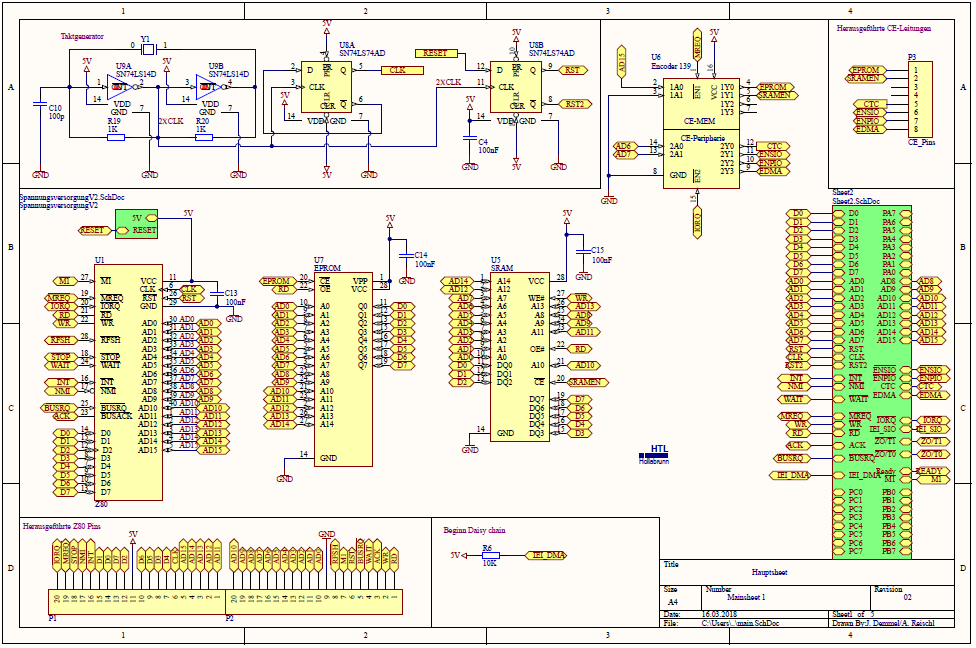
\includegraphics[width=\linewidth]{Reischl/img/z80-gesamt-1}}\qquad
    \subfloat[Mainsheet 2]{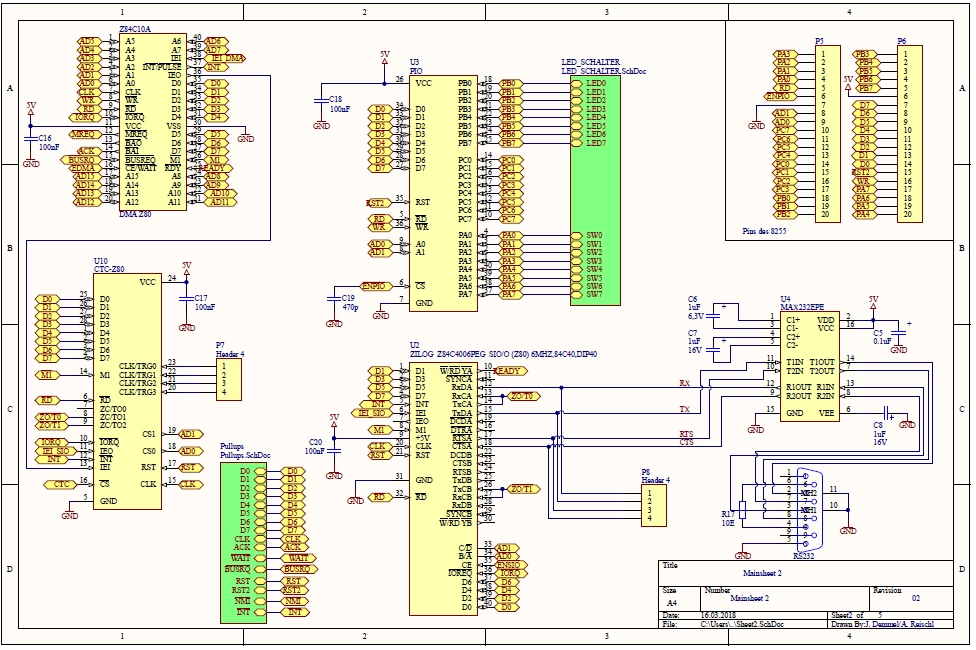
\includegraphics[width=\linewidth]{Reischl/img/z80-gesamt-2}}\qquad
\end{figure}
\begin{figure}[H]
    \ContinuedFloat
    \subfloat[Spannungsversorgung]{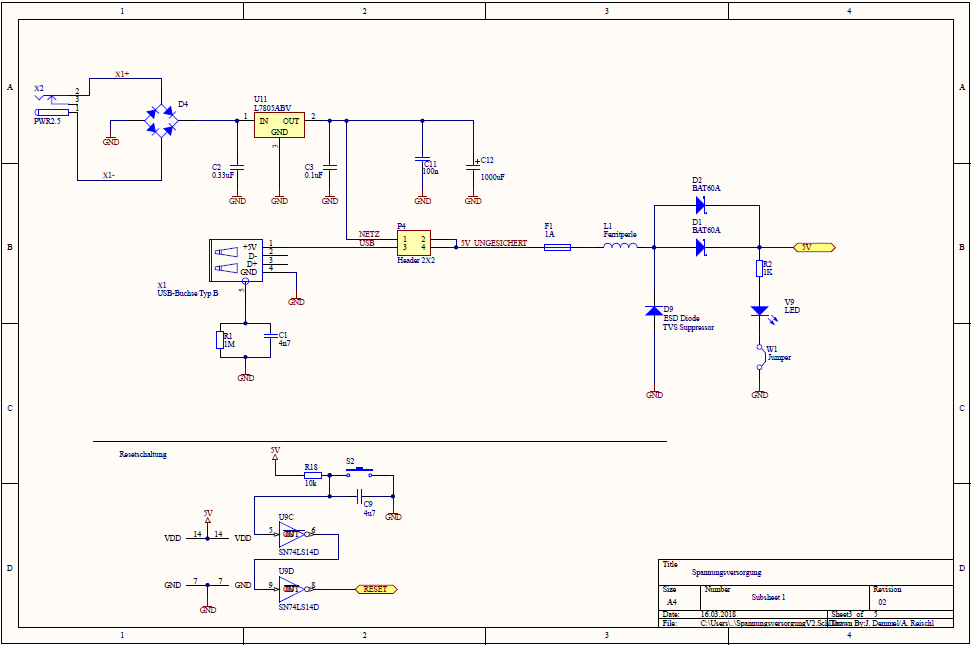
\includegraphics[width=\linewidth]{Reischl/img/z80-gesamt-3}}\qquad
    \subfloat[LED und Schalter (I/O)]{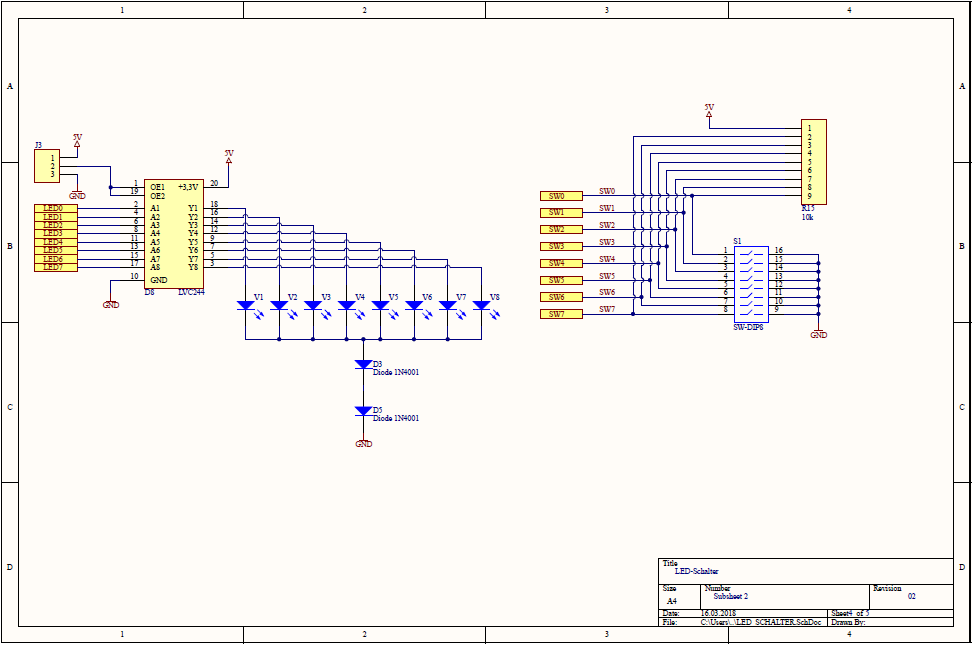
\includegraphics[width=\linewidth]{Reischl/img/z80-gesamt-4}}\qquad
\end{figure}
\begin{figure}[H]
    \ContinuedFloat
    \subfloat[Pull-Ups]{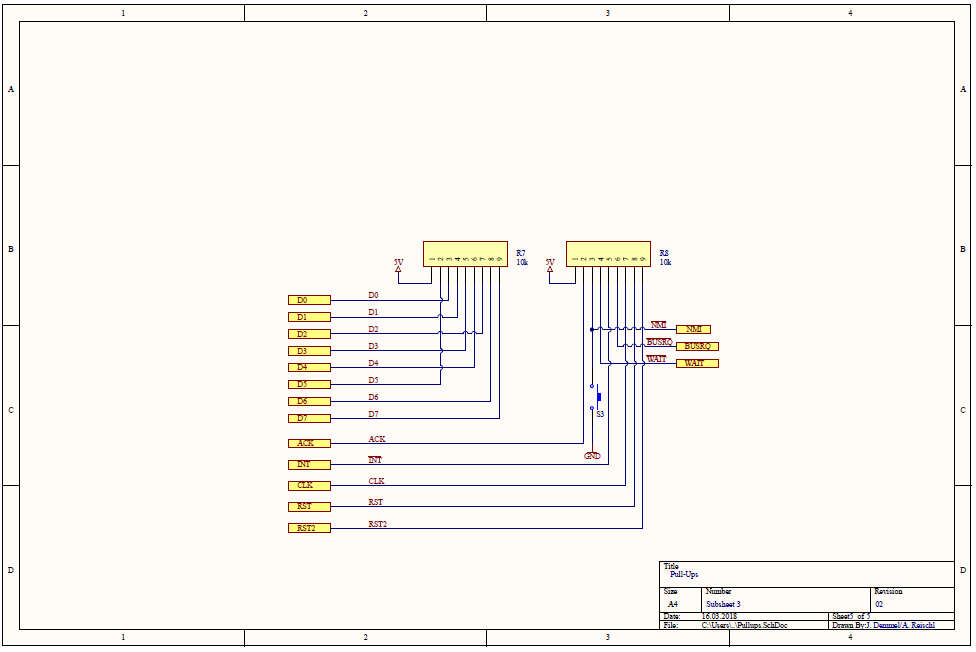
\includegraphics[width=\linewidth]{Reischl/img/z80-gesamt-5}}\qquad
    \caption[Z80 Schematics]{Schematics}
    \label{fig:z80-zeit}
\end{figure}

\subsection{Verbesserungen im Vergleich zur Version 4.5}
\subsubsection{Spannungsversorgung}
Im Vergleich zu den Vorgängerversionen wurde die Spannungsversorgung stark modifiziert. Beim Z80 Minimalsystem V4.5 wurde eine Leiterbahnbreite von unter 25 Mil = 0,64mm für die Versorgungsleitungen vorgesehen, welche bei der Verwendung alter TTL-Komponenten, wo der Stromverbrauch abhängig vom angewendeten Programm 400 bis zu 440 mA beträgt, zu einem Spannungsabfall von 0,6V zwischen Linearregler und 5V Pin der CPU führten. Es konnte das in den Datenblättern der Z80-spezifischen Komponenten vorgegebenen Minimum von 4,75V nicht erreicht werden. Der gemessene Spannungswert an den herausgeführten Pins der CPU ergab eine Spannungsdifferenz von minimal 4,35V zwischen VCC und GND. Bei der aktuellen Version 4.9 sind die Leiterbahnen für 5V und Ground mit mindestens 50 mil Breite ausgeführt, ebenso ist anstelle der Schottky-Diode, welche als zusätzlicher Verpolungsschutz dient, eine Parallelschaltung zweier Schottky-Dioden zur Minimierung der Spannung an der Diode in Verwendung. Als Ergebnis dieser Überdimensionierung erhält man eine Versorgungsspannung von mindestens 4,75V an den Versorgungspins der CPU, auch dann, wenn TTL- anstatt CMOS- oder NMOS-Technologie eingesetzt wird.

Neben sehr vielen kleineren Änderungen sollte auch der Wechsel von Micro USB auf USB Typ B erwähnt werden. Durch diese Änderung wird die mechanische Stabilität des Steckers wesentliche verbessert und dadurch Störfälle minimiert.

\subsubsection{Reset}
Der Reset wurde ursprünglich ohne die Verwendung eines RC-Gliedes zur Stabilisierung des Signals beschaltet, was sehr viele kurze Störimpulse durch das Prellen des Schalters und dadurch einen unvollständigen Reset zur Folge hatte. Nunmehr ergibt ich durch den Kondensator C9 parallel zum Reset-Taster ein für den Ladevorgang eines Kondesators typischer Spannungsverlauf, der einer Exponentialfunktion entspricht und frei von Störimpulsen ist. Mithilfe des Schmitt-Triggers wird eine diskrete Schaltschwelle geschaffen und die Flankensteilheit des Impulses erhöht, sodass dieser für digitale Eingänge nutzbar wird.

\fig{z80-reset-oszi}{Z80 Resetimpuls am Taster S2}{Resetimpuls am Taster S2}{0.75\textwidth}{Reischl/img/z80-reset-oszi}
\fig{z80-reset-cpu-oszi}{Z80 Taktsignal und Reset an der CPU}{Taktsignal und Reset an der CPU}{0.75\textwidth}{Reischl/img/z80-reset-cpu-oszi}

\subsubsection{Taktsignal}
Das Taktsignal wirkt sich nicht negativ auf die Funktion des Minimalsystems aus, jedoch ist das Signal noch verrauscht und die Pegel des Systemtaktes weichen von den Vorgaben des Datenblattes der CPU ab. Diese Vorgaben besagen, dass der Low-Pegel eine Spannung von minimal -0,3V und maximal 0,45V haben darf und der High-Pegel nicht um mehr als -0,6V und +0,3V von der Versorgungsspannung abweichen darf. Abhilfe würde durch die Verwendung von SMD-Widerständen aufgrund geringerer parasitärer Kapazitäten und Induktivitäten und den Wechsel auf schnellere CMOS-Gatter für die Takterzeugung schaffen. Die Gatter vom Typ HCT bzw. AHCT weisen kürzere Schaltzeiten auf, besitzen jedoch die gleichen Schwellen wie die TTL-Gatter vom Typ LS.
\fig{z80-takt-oszi}{Z80 Taktsignal}{Taktsignal}{0.75\textwidth}{Reischl/img/z80-takt-oszi}

% \subsection{Troubleshooting}
% \label{sec:z80-troubleshooting}
% \subsubsection{Spannungsversorgung}
% Im Vergleich zu den Vorgängerversionen wurde die Spannungsversorgung stark modifiziert. Beim Z80 Minimalsystem V4.5 wurde eine Leiterbahnbreite von unter 25 Mil = 0,64mm für die Versorgungsleitungen vorgesehen, welche bei der Verwendung von alter TTL-Komponenten, wo der Stromverbrauch abhängig vom angewendeten Programm 400 bis zu 440 mA beträgt, zu einem Spannungsabfall von 0,6V zwischen Linearregler und 5V Pin der CPU führen. Es kann das in den Datenblättern vorgegebenen Minimum von 4,75V nicht erreicht werden, der gemessene Spannungswert an den herausgeführten Pins der CPU ergibt eine Spannungsdifferenz von minimal 4,35V. Bei der aktuellen Version 4.9 werden die Leiterbahnen für 5V und Ground mit mindestens 50 mil Breite ausgeführt, ebenso wird die Schottky-Diode, welche als zusätzlicher Verpolungsschutz dient, durch eine Parallelschaltung zweier Schottky-Dioden zur Minimierung der Spannung an der Diode ersetzt. Als Ergebnis dieser Überdimensionierung erhält man eine Spannung von mindestens 4,75V an der Versorgung der CPU, auch dann, wenn TTL- anstatt CMOS- oder NMOS-Technologie eingesetzt wird.

% Neben vielen kleineren Änderungen sollte der Wechsel von Micro USB auf USB Typ B erwähnt werden. Durch diese Änderung wird die mechanische Stabilität des Steckers wesentliche verbessert und dadurch Störfälle minimiert.

% \subsubsection{Reset}
% Der Reset wurde ursprünglich ohne die Verwendung von Schmitt-Triggern zur Stabilisierung des Signals beschaltet, was sehr viele kurze Störimpulse durch das Prellen des Schalters zur Folge hatte. Durch die nunmehrige Anwendung eines Kondensators zum Vermeiden von Spannungssprüngen in Kombination mit 2 Schmitt-Trigger-Invertern und einem D-Flip-Flop ergibt sich eine Ladekurve mit einer Zeitkonstante von rund 60ms und daraus ein sauberer Reset-Impuls.
% \fig{z80-reset-oszi}{Z80 Resetimpuls}{Resetimpuls}{0.75\textwidth}{Reischl/img/z80-reset-oszi}

% \subsubsection{Taktsignal}
% Das Taktsignal wirkt sich nicht negativ auf die Funktion des Minimalsystems aus, doch weist es noch immer unerwünschte Impulse und die Pegel des Systemtaktes weichen von den Vorgaben des Datenblattes der CPU ab. Abhilfe würde durch die Verwendung von SMD-Widerständen aufgrund geringerer parasitärer Größen und den Wechsel auf schnellere CMOS-Gatter für die Takterzeugung schaffen. Die Gatter vom Typ HTC bzw. AHCT weisen kürzere Schaltzeiten auf, besitzen jedoch die gleichen Schwellen wie die TTL-Gatter vom Typ LS.
% \fig{z80-takt-oszi}{Z80 Taktsignal}{Taktsignal}{0.75\textwidth}{Reischl/img/z80-takt-oszi}

\subsection{Programmierung}
\label{sec:z80-programmierung}
\subsubsection{Programmierung des EPROMs}
Die Programmierung des EPROMS wird mit einem Programmiergerät vorgenommen. Dieses Programmiergerät vom Typ MiniPRO TL866 wird mittels USB mit einem Computer verbunden. Um die Software MiniPro Programmer V6.1 für das Programmiergerät zu installieren, muss die beigefügte CD ausgeführt werden. Bei der Installation können die Standardeinstellungen übernommen werden. Ist die Installation ausgeführt worden, kann die Programmierung erfolgen. Dafür müssen die Speicherzellen entsprechend der vorgesehenen Adressierung mit HEX Code befüllt werden. Dieser Hex-Code kann entweder aus einem File mit File -> Open geladen werden oder direkt in die Speicherzellen eingetragen werden. Um den EPROM flashen zu können, muss in der Software mit Select IC -> Search and Select der zu programmierende IC ausgewählt werden.  Mit Device -> Program wird mithilfe des über USB mit dem PC verbundenen Programmiergeräts das Programm in den EPROM geschrieben.
\fig{z80-programmierung-eprom}{Z80 EPROM Programmierung - Mini Pro V6.10}{EPROM Programmierung - Mini Pro V6.10}{\textwidth}{Reischl/img/z80-programmierung-eprom}

\subsubsection{Z80 Assembler}
Grundsätzlich kann die Übersetzung des Assemblercodes in Intel HEX-Code von Hand erfolgen. Bei größeren Programmen empfiehlt es sich, einen Assembler zu verwenden, wie etwa das Crossware Embedded Development Studio, welcher sowohl als Assembler als auch als Simulator verwendet werden kann. Da dieser Assembler standardmäßig für die Anwendung mit dem MPF 1B konfiguriert ist, muss die Startadresse auf 0000 statt 1800 geändert werden ebenso wie die Größe des Speichers und die Auswahl des EPROMS als Programmspeichermedium. Bei der Übersetzung des Programms liefert der Assembler ein HEX-File, welches für die Programmierung des EPROMS mit der dafür vorgesehenen Software MiniPro Programmer geeignet ist. Genaue Informationen zu Installation und Anwendung liegen der Software in englischer Sprache bei.

\subsection{Software und Analyse}
\label{sec:z80-software}
\subsubsection{Beschreibung der Hardware}
Eine genaue Beschreibung der Hardware ist dem Kapitel Aufbau des Z80 Minimalsystems und Beschreibung der Baugruppen zu entnehmen.

\subsubsection{Der Von-Neumann Zyklus}
Der von-Neumann-Zyklus, benannt nach dem österreich-ungarischen, später US-amerikanischen Mathematiker János/Johann/John von Neumann, beschreibt den Ablauf der Befehlsverarbeitung in einer entsprechend den Vorschlägen von Neumanns entworfenen Architektur. Diese besteht aus einer Rechenwerk mit der ALU (Arithmethic Logic Unit), einer Control Unit (dem Steuerwerk), einem Bussystem, einem Speicherwerk, welches sowohl Daten als auch Instruktionen gleichwertig speichert und den Ein- und Ausgabeeinheiten. Die Befehlsausführung wird in 5 Schritten vorgenommen:

\begin{enumerate}
    \item \textbf{Instruction Fetch}: Instruktion aus den Programmspeicher in das Befehlsregister laden
    \item \textbf{Instruction Decode}: Der Befehlsdecoder decodiert den HEX-Code aus dem Befehlsregister, sodass der Controller Sequenzer die nötigen Steuersignale erzeugen kann.
    \item \textbf{Operanden Fetch}: Entsprechend dem decodierten Befehl werden, wenn erforderlich, die nötigen Operanden aus dem Speicher geladen.
    \item \textbf{Execute}: Ausführung des Befehls
    \item \textbf{Write Back}: Die erhaltenen Ergebnisse werden, wenn im Befehl enthalten, in die Register oder in den Arbeitsspeicher zurückgeschrieben.
\end{enumerate}
\begin{warning}
    Anmerkung: Für den von-Neumann Zyklus existieren mehrere verschiedene Varianten. Eine Variante beinhaltet das Zurückschreiben der Ergebnisse als fünften Teil, in der zweite Variante ist das Zurückschreiben ein Teil der Ausführung und der letzte Schritt das Laden der Adresse für den nächsten Befehl, also das Aktualisieren des Program Counters. In anderen Varianten wiederum besteht der von-Neumann Zyklus aus nur vier Schritten und endet mit der Ausführung.
\end{warning}

\subsubsection{Vorbereitung zur Analyse der Z80-Befehlsabarbeitung}
\subsubsubsection{Installation der DigiView-Software}
Um die mittels Logikanalysator aufgenommenen Signalverläufe auf einem PC anzeigen zu können bzw. die Analyse durchzuführen, muss das Programm DigiView installiert werden, welche auf der dem Logikanalysator beigelegten Installations-CD enthalten ist. Bei der Installation der Software muss nach der vorgenommenen Installation noch der Treiber für den Logikanalysator nachinstalliert werden. Dies geschieht üblicherweise über die Systemsteuerung, wo als Quelle für den Treiber die CD zu wählen ist.

\subsubsubsection{Kanalkonfiguration in DigiView}
\label{sec:z80-digiview-kanal}
Um die Signale erfassen und analysieren zu können, muss für jeden einzelnen Kanal, also für jeden Eingang des Logikanalysators, eine Bezeichnung vergeben werden. Für die anschließende Analyse muss festgelegt werden, um welche Art von Signal es sich handelt. Grundsätzlich wird zwischen einzelnen Leitungen (Boolean) und zwischen einem Bündel von Leitungen (Bus) unterschieden.

Konfiguration für das Programm PIO Test \#2:
\fig{z80-digiview-kanal}{Z80 DigiView Kanalkonfiguration PIO Test 2}{DigiView Kanalkonfiguration PIO Test 2}{\textwidth}{Reischl/img/z80-digiview-kanal}
\begin{warning}
    Anmerkung: Diese in der Abbildung gezeigte Belegung ist beispielhaft und entspricht nur der Belegung der Kanäle zur Erfassung des Bustimings des Programms PIO\_TEST\#2. Die erfassten Signale bzw. die Auswahl und Belegung der Kanäle unterscheidet sich bei den jeweiligen Programmen, weshalb sie bei jedem Einzelnen separat angeführt ist.
\end{warning}

\subsubsubsection{Festlegung der Triggerbedingung in DigiView}
Für das Auslösen des Aufzeichnungsvorgangs muss wie bei einem Oszilloskop ein Trigger gesetzt werden. Dieser Trigger wird als Hardware Trigger ausgeführt, die Triggerung wird mittels logischer Verknüpfung eines oder mehrerer Kanäle unter dem Menüpunkt Config $\rightarrow$ Trigger erstellt.
\fig{z80-digiview-trigger}{Z80 DigiView Trigger}{DigiView Trigger}{\textwidth}{Reischl/img/z80-digiview-trigger}
Die in der obigen Abbildung dargestellte Trigger-Bedingung besteht aus 3 Elementen: Der erste Teil der Bedingung wird erfüllt, sobald der Kanal Reset, welcher dem Ausgang der Reset-Schaltung des Minimalsystems entspricht, für eine Zeit von mindestens 10us (Minimum: 3 Taktzyklen entspricht 1,61us) LOW ist. Folgt darauf eine positive Flanke und ein HIGH von 10us, so sind auch der 2. und 3. Teil der Bedingung erfüllt, der Trigger wird ausgelöst und die Aufzeichnung startet. Der erste und zweite Teil der Bedingung vermeiden, dass der Logikanalysator auf ein Störsignal triggert, der dritte Teil prüft auf unerwünschte, störungsbedingte Reset-Impulse und ist nicht zwingend erforderlich.

\subsubsection{Verbindung des Logikanalysators mit dem Z80 Minimalsystem}
Der Logikanalysator, welcher in der Laborübung verwendet wird, besitzt 36 Kanäle, die über 2 Stecker mit jeweils 18 Kanälen und 2 Masseverbindungen nach außen geführt werden. Die einzelnen Leitungen besitzen eine festgelegte farbige Markierung, um die Zuordnung zu erleichtern.

Messleitungen/Kanäle des Logikanalysators:
\fig{z80-digiview-logik}{Z80 DigiView Kanäle des Logikanalysators}{DigiView Kanäle des Logikanalysators}{\textwidth}{Reischl/img/z80-digiview-logik}
Entsprechend dieser Zuordnung und der zuvor festgelegten Kanäle müssen die herausgeführten Pins von Adressbus, Datenbus, CE-Logik und der Steuerleitungen des Z80 Minimalsystems mit den Leitungen der einzelnen Kanäle verbunden werden. Die Zuordnung der auf die Stiftleisten herausgeführten Leitungen kann entsprechend dem Aufdruck auf der Platine und den Schaltplänen vorgenommen werden, es sollte aber dringend darauf geachtet werden, dass auch GND (fixe Belegung am Logikanalysator, bezeichnet mit G) verbunden wird.

\subsubsubsection{Belegung der herausgeführten Leitungen auf dem Minimalsystem}
\begin{warning}
    Anmerkung: Um etwaige Fehler bei der späteren Interpretation der Timing Diagramme zu vermeiden, sollte angemerkt werden, dass sämtliche Leitungen für Daten-, Steuer- und Adressbus invertierte Ein- und Ausgänge besitzen.
\end{warning}
\begin{figure}[H]
    \centering
    \subfloat{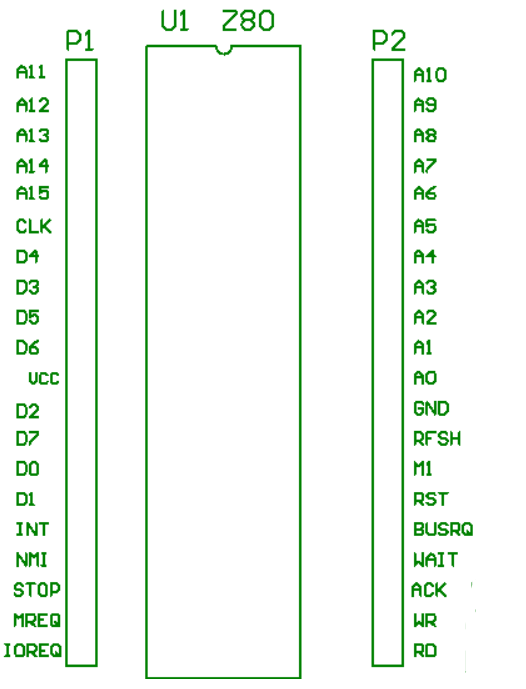
\includegraphics[width=.28\linewidth]{Reischl/img/z80-stiftleiste-1}}\qquad
    \subfloat{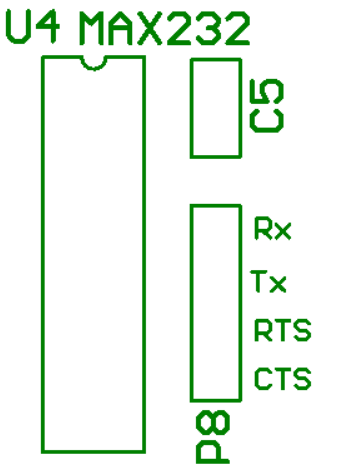
\includegraphics[width=.28\linewidth]{Reischl/img/z80-stiftleiste-2}}\qquad
    \subfloat{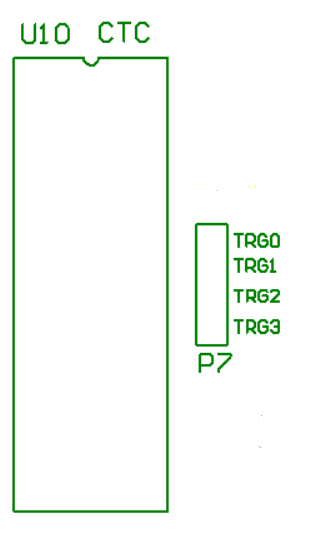
\includegraphics[width=.28\linewidth]{Reischl/img/z80-stiftleiste-3}}\qquad
    \caption[Z80 Belegung der Stiftleisten an CPU, CTC und UART]{Belegung der Stiftleisten an CPU, CTC und UART}
    \label{fig:z80-stiftleiste}
\end{figure}
Wie dem Bild zu entnehmen ist, werden an den Stiftleisten P1 und P2 der gesamte Adress- und Datenbus und die meisten Leitungen des Steuerbusses herausgeführt. An der Stiftleiste P8 werden die Daten- und Steuerleitungen für die RS232-Schnittstelle abgerufen werden. Die Triggerleitungen des CTC sind an der Stiftleiste P7 herausgeführt. Die Stiftleisten P5 und P6 sind mit den Pins des PIO verbunden und nicht beschriftet, da sie im Regelfall nicht verwendet werden. Sollten sie benötigt werden, kann die Belegung den Schematics entnommen werden.

\subsubsection{PIO Testprogramm}
\subsubsubsection{Aufgabenstellung}
Es ist mithilfe eines Logikanalysators der Befehlsablauf einer Von-Neumann-Architektur anhand des Z80 Minimalsystems zu analysieren. Das zu verwendende Programm für den Zilog Z80 lautet auf dem Namen PIO\_TEST\#2. Es liest mithilfe des PIO (8255) die Schalterstellung aus und zeigt diese über die LEDs an. Es soll eine Erfassung des Befehlsablaufes ab dem Reset vorgenommen werden. Anschließend zu analysieren sind vor allem die Instruktionen, die in das Control-Register des PIO geschrieben werden. Weiters soll eine Messung der Zugriffszeiten auf die einzelnen Komponenten des Systems, in diesem Fall auf EPROM und PIO, erfolgen und die Gatterlaufzeit der CE-Logik ermittelt werden.

\subsubsubsection{Source Code}
Das Programm für den Z80 wird in Assemblersprache verfasst. Um das Programm ausführen zu können, muss die Assemblersprache in Hex-Code übersetzt werden und dieser mit einem Programmiergerät in ein EPROM geschrieben werden.
\lstinputlisting[language={[Z80]Assembler}, caption=Z80 PIO Test, label=lst:z80-pio]{Reischl/lst/pio.s}

\subsubsubsection{HEX-Code}
Der hier abgebildete Source Code ist um die Speicheradressen und um den Hex Code der jeweiligen Befehle ergänzt. Abgespeichert wird diese Datei als List File (.lst).
\lstinputlisting[language={[Z80]Assembler}, caption=Z80 PIO Test HEX-Code, label=lst:z80-pio-lst]{Reischl/lst/pio.lst}

\subsubsubsection{Konfiguration des Logikanalysators}
Die Kanalbelegung des Logikanalysators ist der Erläuterung der Bedienung des Logikanalysators in \fref{sec:z80-digiview-kanal} zu entnehmen.

\subsubsubsection{Analyse}
Die Beschreibung der einzelnen Zyklen erfolgt entsprechend der Bezeichnung der einzelnen Marker T, A-D, X und Y. Bei dieser Abbildung wurde ein Marker mit der Bezeichnung Z ergänzt.
\fig{z80-digiview-pio}{Z80 DigiView PIO Test 2 Teil 1}{DigiView PIO Test 2 Teil 1}{\textwidth}{Reischl/img/z80-digiview-pio}
Marker T: Mit dem Reset wurde der Program Counter auf die Adresse 0000 zurückgesetzt. Die Adresse 0000 ist als die erste Adresse des auszuführenden Programms festgelegt, weshalb die CPU einen Opcode Fetch durchführt. Dafür aktiviert die CPU die Leitungen M1 (Machine Cycle One), MREQ (Memory Request) und RD (Read). Da die Leitungen bzw. Die Ein- und Ausgänge von Adress-, Daten- und Steuerbus invertiert sind, werden sie auf Low gesetzt. Die CE-Logik enabled anhand des Memory Requests und des 16. Bits des Datenbusses den EPROM. Im EPROM wird der Inhalt der Speicherzelle mit der Adresse 0000 an den Datenbus gelegt. Vom Datenbus wird der Opcode 3E in das Befehlsregister geladen und vom Befehlsdecoder decodiert. Der Befehl mit dem Opcode 3E ist ein 8-Bit-Transferbefehl, welcher einen Wert aus dem Speicher in den Akkumulator lädt.

Marker A: Da die CPU auch die Verwendung dynamischer RAMs unterstützt und deren Speicherinhalt flüchtig ist, wird alle 5μs ein Refresh aufgelöst, um die Speicherzellen aufzufrischen und somit den Speicherinhalt zu halten. Diese Funktion wird standardmäßig ausgeführt, findet aber beim Z80 Minimalsystem keine Anwendung.

Marker B: Nach dem Refresh wird der Inhalt des Program Counters wiederhergestellt, um 1 erhöht und an den Datenbus gelegt. Um den ersten Operanden mittels Speicher-Lesezugriff aus dem EPROM zu holen, wird der Inhalt des Befehlszählers an den Adressbus gelegt und die CPU gibt einen Memory Request für einen Datenaustausch mit dem Speicher und ein Read für einen Lesevorgang aus. Anhand des Memory Requests und des 16. Bits des Adressbusses, welches 0 ist, generiert die CE-Logik am Ausgang ein CE-Signal für den EPROM. Dieser legt nach einigen Nanosekunden (Access Time) den Inhalt der Speicherzelle, 99, an den Datenbus. Von dort werden die Daten in den Akkumulator geladen. Die in den Akku geladene Konstante ist für die Konfiguration des PIOs (8255) bestimmt. Der Port B des Parallel Input/Output Controllers soll als Output für die Ausgabe über LED konfiguriert werden, Port A als Input für das Einlesen der Schalterstellungen des DIL-Schalters, als Modus wird der Mode 0 gewählt. Die Ausführung des Befehls ist abgeschlossen, wenn der Befehlszähler inkrementiert ist und die Adresse für den nächsten Befehl am Adressbus anliegt.

Marker C: Mit diesem Zyklus wird ein Opcode Fetch durchgeführt. Der dabei erhaltene Opcode D3 entspricht einem Ausgabebefehl für die Peripherie.

Marker D: Nach dem Inkrementieren des Program Counters wird der Inhalt am Adressbus ausgegeben. Von dieser Adresse soll der erste Operand, die Zieladresse für den Ausgabebefehl geladen werden. Mittels Speicher-Lesezugriff wird die Adresse 83 vom EPROM geholt und im W-Register abgelegt.

Marker X: Nachdem sowohl die Adresse als auch die zu übertragenden Daten aus dem Speicher geholt wurden, kann die Ausgabe der Daten und damit die Konfiguration des PIO erfolgen. Dazu wird die Adresse 83 an den Adressbus gelegt. Die Adressen für die Peripherie sind immer nur 8 Bit breit, der Datenbus jedoch 16 Bit. Somit entspricht das Low Byte der Adresse 83 und das nicht verwendete High Byte wird mit den momentan auf dem Datenbus befindlichen Daten beaufschlagt. Dadurch ergibt sich die irreführende Adresse 9983. Für das Beschreiben des Control Registers des PIOs werden von der CPU die Signale IOREQ (I/O Request) und WR (Write) erzeugt. Anhand der Adresse und der Steuersignale enabled die CE-Logik nach einer Laufzeit den PIO und die Datenübertragung kann stattfinden.

Marker Y: Nach dem Inkrementieren des Program Counters wird die dabei erhaltene Adresse 0004 an den Adressbus gelegt und ein Opcode Fetch durchgeführt. Der am Datenbus anliegende Befehl mit dem Hex-Code DB ist für das Auslesen von Peripherieeinheiten und das anschließende Speichern der ausgelesenen Information im Akku zuständig.

\begin{warning}
    Anmerkung: Nach jedem Zugriff auf den Programmcode, sei es zum Abruf des Opcodes oder zum Laden von Operanden, wird der Program Counter inkrementiert. Beim nächsten Zugriff auf den Programmcode wird der Inhalt des PC dann auf dem Adressbus ausgegeben.
\end{warning}

\fig{z80-digiview-pio-2}{Z80 DigiView PIO Test 2 Teil 2}{DigiView PIO Test 2 Teil 2}{\textwidth}{Reischl/img/z80-digiview-pio-2}
Marker A: Mittels Speicher-Lesezugriff wird die Adresse 83 zur Abfrage der Daten im Control Register des PIO aus dem EPROM geladen.

Marker B: Für die Ausführung des Befehls legt die CPU die Adresse 83 an den Datenbus. Für die Abfrage der Daten erzeugt sie einen I/O Request und ein Read und die CE-Logik enabled den PIO. Der PIO legt nun den Inhalt des Control Registers an den Datenbus, von wo die CPU die Daten in den Akku lädt.

Marker C: Mit dem Opcode Fetch wird wieder der Opcode DB in das Befehlsregister der CPU geladen.

Marker D: Die Adresse 80 wird als erster Operand aus dem EPROM geholt.

Marker X: Das Portregister A des PIO wird über den Adressbus adressiert und die Daten am Datenbus ausgegeben. Von dort werden sie in den Akku geladen. Die Daten 0A entsprechen der Schalterstellung des 8-fach DIL-Schalters.

Marker Y: Mit dem Opcode Fetch wird der Opcode D3 aus dem EPROM geladen. Der sich im Befehlsregister bzw im Befehlsdecoder befindliche Befehl D3 entspricht einem Ausgabebefehl für die Peripherie.

\fig{z80-digiview-pio-3}{Z80 DigiView PIO Test 2 Teil 3}{DigiView PIO Test 2 Teil 3}{\textwidth}{Reischl/img/z80-digiview-pio-3}
Marker A: Die Zieladresse 81 für die Ausgabe wird aus dem EPROM geladen.

Marker B: Der Port B des PIO wird mit 81 adressiert und die Daten an den EPROM übermittelt. Nun wird die hexadezimale Zahl 0A binär über das LED-Array ausgegeben.

Marker C: Die CPU führt einen Opcode Fetch durch, bei dem der Befehl mit dem Opcode C3 geladen wird. Dieser steht für einen Sprungbefehl auf eine durch den Programmierer vorzugebende Adresse.

Marker D: Da die Adresse für den Sprung 16 Bit groß ist, der Datenbus aber nur 8 Bit breit, wird die Adresse in zwei Schritten geladen. Im ersten Schritt wird das Low Byte der Sprungadresse mit einem Speicher-Lesezugriff aus dem EPROM geholt und im W-Register abgelegt.

Marker X: Das High Byte wird in einem weiteren Speicher-Lesezugriff aus dem EPROM geholt und im Z-Register abgelegt. Nun kann der Sprung durchgeführt werden, also der Inhalt des WZ-Registers in den Befehlszähler geladen werden.

Marker Y: Nach dem Sprung legt der Sequencer den Inhalt des Program Counters, die Adresse 0006, an den Adressbus und die CPU führt einen Opcode Fetch durch. Geladen wird der Opcode DB, der Daten von der Peripherie abfragt.

\fig{z80-digiview-pio-4}{Z80 DigiView PIO Test 2 Teil 4}{DigiView PIO Test 2 Teil 4}{\textwidth}{Reischl/img/z80-digiview-pio-4}
Marker A: Für die Abfrage der Daten wird die 8-Bit-Adresse 80 aus dem EPROM geladen.

Marker B: Die Schalterstellung des 8-fach DIL-Schalters wird vom Portregister A des PIO mit der Adresse 80 abgerufen und in den Akkumulator geladen.

Marker C: die CPU führt einen Opcode Fetch durch und lädt dabei den Befehl mit dem Opcode D3, welcher Daten an die Peripherie ausgibt.

Hier wird die Analyse beendet, da keine neuen Befehle mehr ausgeführt werden, sondern in einer Endlosschleift der Port A des PIO ausgelesen und die erhaltene Information über den Port B wieder ausgegeben wird.

\subsubsubsection{Zugriffszeiten auf den EPROM laut Datenblatt}
Auszug aus dem Datenblatt (ST M27256-1)
\fig{z80-eprom-access}{Z80 Datenblattauszug EPROM}{Datenblattauszug EPROM \cite{z80:eprom}}{0.75\textwidth}{Reischl/img/z80-eprom-access}
$t_{ELGV}$ = 200 ns maximal
$t_{GLQV}$ = 75 ns maximal

\subsubsubsection{Ermittlung der Zugriffszeit auf den EPROM}
\fig{z80-eprom-access-real}{Z80 Messung Zugriffszeit EPROM}{Messung Zugriffszeit EPROM}{\textwidth}{Reischl/img/z80-eprom-access-real}
Zu den Zugriffszeiten der CPU auf den RAM können folgende Aussagen getroffen werden:

T(X)= 5,3550$\mu$s; T(A)=5,5950$\mu$s; T(B)=5,6150$\mu$s; T(C)=5,6300$\mu$s; T(D)=5,6650$\mu$s

Durch diese Messwerte ergibt sich eine Gesamtzugriffszeit vom Anlegen der Adresse der Speicherzelle an den Adressbus bis zur Ausgabe des Inhalts der Speicherzelle auf den Datenbus eine Zeitspanne von 310ns.   Die Gatterlaufzeit der CE-Logik, also die Zeitspanne zwischen dem Erzeugen des Memory Requests und des Reads und dem Selektieren des EPROMs, beläuft sich auf 15ns. Im EPROM selbst kommt es zu einer Laufzeit von 25ns, was der Zugriffszeit entspricht. Da die Maximaldauer zwischen dem Enablen und dem Ausgeben der Daten mit maximal 200ns bzw. 75ns größer ist als die gemessenen 50ns bzw. 25ns, werden diese Vorgaben eingehalten.

\subsubsubsection{Zugriffszeit auf den PIO}
\fig{z80-pio-access-read}{Z80 Messung Zugriffszeit PIO}{Messung Zugriffszeit PIO}{\textwidth}{Reischl/img/z80-pio-access-read}
Zeiten der einzelnen Messpunkte:

T(A)= 36,300$\mu$s;  T(B)=36,8200$\mu$s; T(C)=36,8450$\mu$s; T(D)=36,8950$\mu$s; T(X)=36,9300$\mu$s

Die gesamte Zugriffszeit vom Anlegen der Adresse des Port A des PIO bis zur Ausgabe der Schalterstellung auf den Datenbus ergibt sich zu 630ns. Vor der positiven Taktflanke bis zum Ausgabezeitpunkt der Steuersignale vergehen 25ns, die Chipselect-Logik besitzt eine Gatterlaufzeit von 50ns. Die Reaktionszeit des PIO vom Zeitpunkt der Auswahl durch die CE-Logik bis zum Anlegen der momentanen Schalterstellung beträgt 35ns. Im Datenblatt wird dafür ein Zeitraum von maximal 120ns angegeben, in dem die Daten gültig sein müssen, somit werden die Grenzwerte eingehalten.

\subsubsection{Programm PIO\_RAM\_COUNTER}
\subsubsubsection{Aufgabenstellung}
Auf dem Z80 Minimalsystem ist das Programm PIO\_RAM\_COUNTER auszuführen. Mittels Logikanalysator ist ein Timing-Diagramm aufzuzeichnen, welches anschließend analysiert werden soll. Zusätzlich zur Analyse ist eine Messung der Zugriffszeit der CPU auf den RAM durchzuführen.

\subsubsubsection{Konfiguration des Logikanalysators}
Die Belegung der Kanäle für die Aufzeichnung und die Analyse des Timing-Diagrammes des Programmes PIO\_RAM\_COUNTER sieht folgendermaßen aus:
\fig{z80-digiview-ram-kanal}{Z80 DigiView Kanalkonfiguration PIO RAM Counter}{DigiView Kanalkonfiguration PIO RAM Counter}{\textwidth}{Reischl/img/z80-digiview-ram-kanal}

\subsubsubsection{Assemblercode}
\lstinputlisting[language={[Z80]Assembler}, caption=Z80 PIO\_RAM\_COUNTER, label=lst:z80-ram]{Reischl/lst/PIO_RAM_COUNTER.s}

\subsubsubsection{HEX-Code}
\lstinputlisting[language={[Z80]Assembler}, caption=Z80 PIO\_RAM\_COUNTER HEX-Code, label=lst:z80-ram-lst]{Reischl/lst/PIO_RAM_COUNTER.lst}

\subsubsubsection{Funktionsbeschreibung}
Am Beginn der Ausführung wird der PIO initialisiert. Anschließend wird die Adresse des SRAMs in das HL Register geschrieben, der Inhalt der adressierten Zelle wird in den Akku geladen, über die LEDs ausgegeben und anschließend inkrementiert. Nachdem der Wert in der mittels HL Register adressierten Speicherzelle um 1 erhöht wurde, wird eine Warteschleife aufgerufen, welche eine Wartezeit von 0,5 Sekunden bewirkt, bevor die Schleife von vorne beginnt und der aktuelle Zählerstand wieder ausgegeben und inkrementiert wird. Die Warteschleife besteht aus 2 ineinander verschachtelten Zählschleifen. Jede der Zählschleifen dekrementiert einen Registerinhalt von ursprünglich 255 (FF) solange bis dieser gleich 0 ist und der Sprung zum Beginn der Schleife nicht mehr durchgeführt wird.

\subsubsubsection{Analyse}
\fig{z80-digiview-ram-1}{Z80 DigiView PIO RAM Counter Teil 1}{DigiView PIO RAM Counter Teil 1}{\textwidth}{Reischl/img/z80-digiview-ram-1}
Marker T: Mit dem ersten Takt nach dem Reset liegt am Adressbus die Adresse 0000 an und die CPU führt einen Opcode Fetch durch. Der erhaltene Opcode F3 bewirkt eine Sperre aller Interrupts.

Marker A: Da der Sperrvorgang der Interrupts nur einen Zyklus lang ist, wird bereits im nächsten Zyklus ein erneuter Opcode Fetch durchgeführt. Der Befehl mit dem hexadezimalen Opcode 31 ist ein 16-Bit-Transferbefehl, in diesem Fall für das Setzen des Stackpointers.

Marker B: Mittels Speicher-Lesezugriff wird vom EPROM das Low Byte des Stackpointers geladen.

Marker C: Ein weiterer Speicher-Lesezugriff holt aus dem Speicher das High Byte des Stackpointers.

Marker D: Es wird ein Opcode Fetch durchgeführt. Der Befehl mit dem Opcode 3C ist ein Sprungbefehl mit im Befehl angegebener Sprungadresse.

Marker X: Das Low Byte der Sprungadresse wird mittels Speicher-Lesezugriff aus dem EPROM geholt und im W-Register abgelegt.

Marker Y: In einem weiteren Speicher-Lesezugriff wird das High Byte der Sprungadresse vom EPROM in das Z-Register geladen. Anschließend wird der Inhalt vom WZ-Registerpaar in den Program Counter geladen.

\fig{z80-digiview-ram-2}{Z80 DigiView PIO RAM Counter Teil 2}{DigiView PIO RAM Counter Teil 2}{\textwidth}{Reischl/img/z80-digiview-ram-2}
Marker A: Die CPU führt einen Opcode Fetch durch. Der enthaltene Befehl mit dem Opcode 3E ist ein Transferbefehl (Load), welcher eine durch den Programmierer festgelegte Zahl in den Akku der CPU lädt.

Marker B: Aus der Zelle mit der Adresse 0101 wird mittels Speicher-Lesezugriff die Konfiguration des PIO, 99, in den Akku geladen.

Marker C: Mit Beginn des nächsten Zyklus wird ein Opcode Fetch durchgeführt, bei dem aus der Speicherzelle 0102 der Befehl mit dem Opcode D3 geholt wird. Dieser Befehl ist ein Ausgabebefehl für die Peripherie.

Marker D: Als erster Operand wird die Adresse 83 vom EPROM in die CPU geladen.

Marker X: Die Ausgabe der Daten an die Peripherie wird durchgeführt, 99 wird an die Adresse 83 übermittelt.

Marker Y: Der nächste Zyklus beginnt mit einem Instruction Fetch, bei welchem der Opcode 3E geladen wird. Es handelt sich dabei um einen Transferbefehl, welcher im Programmcode festgelegte Daten in den Akkumulator lädt.

\fig{z80-digiview-ram-3}{Z80 DigiView PIO RAM Counter Teil 3}{DigiView PIO RAM Counter Teil 3}{\textwidth}{Reischl/img/z80-digiview-ram-3}
Marker A: Für die Ausführung des Transfers benötigt die CPU die zu übertragenden Daten, welche mittels Speicher-Lesezugriff vom EPROM geholt werden.

Marker B: Beim darauffolgenden Opcode Fetch wird der Befehl 21 geladen. Bei diesem Befehl handelt es sich um einen 16-Bit-Transferbefehl, bei dem durch den Programmierer festgelegte Daten in das HL-Registerpaar geladen werden.

Marker C: Mittels Speicher-Lesezugriff werden die ersten 8 Bit bzw. das Low Byte, 00, über den Datenbus in das L-Register geladen.

Marker D: Das High Byte, 80, und somit der Inhalt des H-Registers wird ebenfalls an sein Ziel übermittelt.

Marker X: Der bei diesem Opcode Fetch übermittelte Befehl 77 ist ein Transferbefehl, bei dem der Inhalt des Akkus in die Speicherzelle geladen wird, welche im HL-Registerpaar adressiert wird.

Marker Y: Am Adressbus liegt 8000, der Inhalt des HL-Registerpaares, an. Die CPU holt mittels Speicher-Lesezugriff 01 vom RAM. Dabei handelt es sich um den ersten Zählerstand des Zählers, der später initialisiert wird.

\fig{z80-digiview-ram-4}{Z80 DigiView PIO RAM Counter Teil 4}{DigiView PIO RAM Counter Teil 4}{\textwidth}{Reischl/img/z80-digiview-ram-4}
Marker A: Ein Opcode Fetch wird durchgeführt. Der vom EPROM über den Datenbus ausgegebene Befehl besitzt den Opcode 7E. Bei dem Befehl handelt es sich um einen Transferbefehl, bei dem die mit dem HL-Registerpaar adressierte Speicherzelle in den Akku geladen wird.

Marker B: Die im HL-Register enthaltene Adresse, 8000 (welches die erste Adresse im RAM darstellt), wird an den Adressbus angelegt und mittels Speicher-Lesezugriff auf den RAM wird von dort der Inhalt der adressierten Zelle, 01, an den Datenbus angelegt und in den Akku geschrieben.

Marker C: Für die Ausführung des nächsten Befehles wird di ein Opcode Fetch durchgeführt. Der geladene Befehl, der Inhalt der Speicherzelle 010B, ist ein Ausgabebefehl mit dem Opcode D3, welcher den Inhalt des Akkus an eine im Programm festgelegte Adresse sendet.

Marker D: Um die Zieladresse 81 zu erhalten, wird mittels Speicher-Lesezugriff der erste Operand aus dem EPROM geholt.

Marker X: Für die Ausgabe des aktuellen Zählerstandes über das LED-Array wird der Port B des PIO mit 81 adressiert und die zuvor eingelesene Schalterstellung am Adressbus ausgebeben.

Marker Y: Es findet ein Opcode Fetch statt, bei dem der Opcode 34 aus dem EPROM ausgelesen wird. Dieser Arithmetikbefehl inkrementiert den mittels HL-Register adressierten Inhalt einer Speicherzelle um 1.

\fig{z80-digiview-ram-5}{Z80 DigiView PIO RAM Counter Teil 5}{DigiView PIO RAM Counter Teil 5}{\textwidth}{Reischl/img/z80-digiview-ram-5}
Marker A: Mit einem Speicher-Lesezugriff auf den RAM liest die CPU den Inhalt der Speicherzelle 8000 des SRAMs, 01 aus um ihn zu inkrementieren.

Marker B: Der um 1 erhöhte neue Inhalt der Speicherzelle wird mittels eines Speicher-Schreibzugriffes in die selbe Speicherzelle des RAMs zurückgeschrieben.

Marker C: Beim Opcode Fetch wird der Befehl CD geladen. Bei diesem Befehl handelt es sich um ein Call, den Aufruf eines Unterprogramms mit im Programmcode festgelegter Sprungadresse.

Marker D: Nach einem Refresh-Zyklus wird aus dem Speicher die Sprungadresse für den Aufruf des Unterprogramms aus dem EPROM geladen. Die Adresse ist 16 Bit lang und wird nach dem Big Endian Format in 2 Teile geteilt, deshalb wird in diesem Schritt das Low Byte in das W-Register geladen.

Marker X: Der 2. Teil der Sprungadresse, das High Byte, wird in einem weiteren Speicher-Lesezugriff aus dem EPROM geladen. Die Adresse lautet 0114 und dient für den Aufruf der Warteschleife.

Marker Y: Um nach der Ausführung des Unterprogramms wieder in den Hauptspeicher zurückkehren zu können, muss eine Rücksprungadresse im Stack abgelegt werden. Dieser Stack befindet sich im obersten Adressbereich des RAMs, wo die Daten ausgehend von der höchstwertigen Adresse absteigend abgelegt werden. Die Rücksprungadresse ist 16 Bit groß, deshalb wird in diesem Schritt lediglich das Low Byte auf den Stack geschrieben.

\fig{z80-digiview-ram-6}{Z80 DigiView PIO RAM Counter Teil 6}{DigiView PIO RAM Counter Teil 6}{\textwidth}{Reischl/img/z80-digiview-ram-6}
Marker A: In einem weiteren Speicher-Schreibzugriff wird auch das High Byte in den Stack geladen und anschießend das Unterprogramm aufgerufen, indem der Program Counter mit der ersten Adresse des Unterprogramms, 0114, beschrieben wird.

Marker B: Am Beginn des Unterprogramms wird ein Opcode Fetch durchgeführt. Bei diesem Vorgang wird der Opcode 16 in den Decoder geladen. Es handelt sich dabei um einen Transferbefehl, der durch den Programmierer vorgegebenen Daten in das D-Register lädt.

Marker C: Mit einem Speicher-Lesezugriff werden die Daten (FF) aus dem EPROM in das D-Register geschrieben.

Marker D: Im nächsten Zyklus wird ein Opcode Fetch durchgeführt, bei dem der Opcode 1E geladen wird. Dieser Befehl ist ein Transferbefehl und bewirkt, dass ein im Speicher festgelegter Wert in das E-Register geladen wird.

Marker X: In einem Speicher-Lesezugriff wird der Wert FF aus der Speicherzelle mit der Adresse 0115 in das E-Register geladen.

Marker Y: Nach dem abgeschlossenen Datentransfer wird ein Opcode Fetch durchgeführt. Der erhaltene Befehl 1D ist ein Arithmetikbefehl, der den Inhalt des E-Registers um 1 dekrementiert.

\fig{z80-digiview-ram-7}{Z80 DigiView PIO RAM Counter Teil 7}{DigiView PIO RAM Counter Teil 7}{\textwidth}{Reischl/img/z80-digiview-ram-7}
Marker A: Es folgt der nächste Opcode-Fetch. Dabei wird der Befehl mit dem Opcode C2 geladen. Bei diesem Befehl handelt es sich um einen bedingten Sprung, der solange stattfindet, solange das Ergebnis des vorherigen Befehls ungleich Null ist.

Marker B: Um den bedingten Sprung ausführen zu können, muss die Adresse, die in den Program Counter geladen werden soll, aus dem Speicher geholt und im WZ-Registerpaar abgelegt werden. Bei der Adresse handelt es sich um eine 16-Bit-Adresse, daher muss die Abfrage in 2 Schritten erfolgen. Mit diesem Schritt wird das Low Byte geladen.

Marker C: Im 2. Teil des Ladevorganges Wird das High Byte der Sprungadresse geladen. Nun kann der Sprung überprüft und vorgenommen werden, indem bei Erfüllung der Bedingung die Adresse im WZ-Registerpaar in den Befehlszähler geladen wird.

Marker D: Die innere Schleife der Warteschleife beginnt von Neuem, indem mittels Opcode Fetch der Befehl zum Dekrementieren des E-Registers aus dem Speicher geladen und decodiert wird.

Alle weiteren Vorgänge des aufgezeichneten Signals sind Teil der Warteschleife. Die vorkommenden Befehle gleichen den in den letzten 8 Punkten beschriebenen Befehlen, lediglich der Rücksprung vom Unterprogramm zurück in das Hauptprogramm würde einen Neuheitswert darstellen. Dieser Vorgang konnte allerdings nicht aufgezeichnet werden, da es mit dem verwendeten Logikanalysator nicht möglich ist, Vorgänge über mehr als 50 ms aufzuzeichnen und die Warteschleife rund 500 ms lang ist.

\subsubsection{Programm CTC\_BLINKY\_Interrupt}
\subsubsubsection{Aufgabenstellung}
Mithilfe des Z80 Minimalsystems ist das Programm CTC\_Blinky\_Interrupt auszuführen und das Timing aufzuzeichnen. Dafür ist ein Logikanalysator zu verwenden. Nachdem das Programm vom Reset an aufgezeichnet worden ist, ist das erfasste Timing zu analysieren und eine Zugriffszeitmessung auf den CTC durchzuführen.

\subsubsubsection{Konfiguration des DigiView Logikanalysators}
\fig{z80-digiview-ctc-kanal}{Z80 DigiView Kanalkonfiguration CTC Blinky Interrupt}{DigiView Kanalkonfiguration CTC Blinky Interrupt}{\textwidth}{Reischl/img/z80-digiview-ctc-kanal}

\subsubsubsection{Source Code}
\lstinputlisting[language={[Z80]Assembler}, caption=Z80 CTC\_BLINKY\_Interrupt, label=lst:z80-ctc]{Reischl/lst/CTC_BLINKY_Interrupt.s}

\subsubsubsection{HEX-Code}
\lstinputlisting[language={[Z80]Assembler}, caption=Z80 CTC\_BLINKY\_Interrupt HEX-Code, label=lst:z80-ctc-lst]{Reischl/lst/CTC_BLINKY_Interrupt.lst}

\subsubsubsection{Funktionsbeschreibung}
Das Programm besteht aus einem Hauptprogramm und einer Interrupt Service Routine. Im Hauptprogramm werden alle Interrupts disabled und der PIO und der CTC konfiguriert, anschließend wird ein Interrupt im Modus 2 konfiguriert und Interrupts wieder aktiviert. Ist die Konfiguration abgeschlossen, läuft eine Endlosschleife. Die Interrupt Service Routine verwendet den 1. Kanal des CTC als Zähler, welcher viermal pro Sekunde die LEDs toggelt.

\subsubsubsection{Analyse}
\begin{warning}
    Anmerkung: Die Analyse dieses Programms beschränkt sich auf die Konfiguration des CTC.
\end{warning}
\fig{z80-digiview-ctc-1}{Z80 DigiView CTC Blinky Interrupt Teil 1}{DigiView CTC Blinky Interrupt Teil 1}{\textwidth}{Reischl/img/z80-digiview-ctc-1}
Marker A: Die CPU führt einen Opcode Fetch durch. Der geladene Opcode 3E steht für einen 8-Bit-Transferbefehl.

Marker B: Mittels Speicher-Lesezugriff wird der erste Operand aus dem Speicher geholt.

Marker C: Der nächste Zyklus ist ein Opcode Fetch, wo der Befehl D3, ein Ausgabebefehl für die Peripherie, geladen wird.

Marker D: Der erste Operand, die Zieladresse 00 für die Ausgabe, wird aus dem Speicher eingelesen.

Marker Y: Die Ausgabe der Daten an die Adresse 00 erfolgt. Dort wird die Konfiguration A5 in das Steuerregister des Kanals 0 geschrieben.

Marker X: Bei diesem Opcode Fetch wird ein Transferbefehl geladen, welcher für das Laden von Daten aus dem Speicher in den Akku zuständig ist.

\fig{z80-digiview-ctc-2}{Z80 DigiView CTC Blinky Interrupt Teil 2}{DigiView CTC Blinky Interrupt Teil 2}{\textwidth}{Reischl/img/z80-digiview-ctc-2}
Marker A: Mittels Speicher-Transferbefehl wird der Wert FF aus dem EPROM geholt. Dabei handelt es sich um die Zeitkonstante für den Timer, es müssen also 256 (Prescaler) x 256 (Zeitkonstante) = 65536 Takte vergehen, bis ein Interrupt ausgelöst wird.

Marker B: Es wird ein Opcode Fetch durchgeführt, bei welchem der Opcode D3 geladen wird. Dieser Opcode bewirkt eine Ausgabe von Daten an die Peripherie.

Marker C: Der erste Operand, die Zieladresse 00, wird aus dem EPROM geladen.

Marker D: Der Ausgabebefehl wird ausgeführt und somit das Zeitkonstantenregister des Kanal 0 des CTC konfiguriert.

Marker X: Nach Abschluss der Konfiguration wird ein Opcode Fetch durchgeführt, wodurch 3E, ein Speicher-Transferbefehl geladen wird.

Marker Y: Die Konfiguration A8 des Interrupt Vector Register wird mittels Speicher-Lesezugriff aus dem EPROM geholt.

\fig{z80-digiview-ctc-3}{Z80 DigiView CTC Blinky Interrupt Teil 3}{DigiView CTC Blinky Interrupt Teil 3}{\textwidth}{Reischl/img/z80-digiview-ctc-3}
Marker A: Mit diesem Zyklus wird ein Opcode Fetch) durchgeführt und D3 geladen. D3 ist der Opcode eines Ausgabebefehls für die Peripherie.

Marker B: Um die Daten aus dem Akku adressieren zu können, muss aus dem EPROM der Operand, die Zieladresse 00, geholt werden.

Marker C: Die Ausgabe der Daten und somit die Konfiguration des Interrupt Vector Registers erfolgt.

Somit ist die Konfiguration abgeschlossen.

\subsubsection{Programm CTC\_Counter}
\subsubsubsection{Source Code}
\lstinputlisting[language={[Z80]Assembler}, caption=Z80 CTC\_Counter, label=lst:z80-ctc-cnt]{Reischl/lst/CTC_Counter.s}

\subsubsubsection{HEX-Code}
\lstinputlisting[language={[Z80]Assembler}, caption=Z80 CTC\_Counter HEX-Code, label=lst:z80-ctc-cnt-lst]{Reischl/lst/CTC_Counter.lst}

\subsubsection{Programm SIO\_V24\_Echo\_Interrupt}
\subsubsubsection{Source Code}
\lstinputlisting[language={[Z80]Assembler}, caption=Z80 SIO\_V24\_Echo\_Interrupt, label=lst:z80-sio]{Reischl/lst/SIO_V24_Echo_Interrupt.s}

\subsubsubsection{HEX-Code}
\lstinputlisting[language={[Z80]Assembler}, caption=Z80 SIO\_V24\_Echo\_Interrupt HEX-Code, label=lst:z80-sio-lst]{Reischl/lst/SIO_V24_Echo_Interrupt.lst}

\subsubsubsection{Funktionsbeschreibung}
Das Programm konfiguriert zuerst SIO, PIO und CTC und versendet dann über den UART, welcher auf eine Baudrate von 9600 Baud konfiguriert wurde, einen String (Z80 DEMO V1.0). Wird von einem Terminal ein Zeichen an das Minimalsystem gesendet, antwortet es mit dem gleichen Zeichen. Dies geschieht mit einem Interrupt, welcher durch den Kanal A des SIO ausgelöst wird. Weiters bewirkt das Auslösen eines Interrupts ebenfalls das Versenden eines Strings (NMI).

\subsubsection{Programm SIO\_V24\_Echo\_Polling}
\subsubsubsection{Source Code}
\lstinputlisting[language={[Z80]Assembler}, caption=Z80 SIO\_V24\_Echo\_Polling, label=lst:z80-sio-poll]{Reischl/lst/SIO_V24_Echo_Poll.s}

\subsubsubsection{HEX-Code}
\lstinputlisting[language={[Z80]Assembler}, caption=Z80 SIO\_V24\_Echo\_Polling HEX-Code, label=lst:z80-sio-poll-lst]{Reischl/lst/SIO_V24_Echo_Poll.lst}

\subsubsubsection{Funktionsbeschreibung}
Das Programm gleicht in seiner Funktion dem Programm SIO\_V24\_Echo\_Interrupt, jedoch wird das Rücksenden der Zeichen nicht durch eine Interrupt Service Routine realisiert, sondern durch das regelmäßige Abfragen des Eingangs.
